\section{Integration of ordinary differential equations}
\thispagestyle{plain}

Our aim is solving an ordinary differential equation (ODE) 
$\partial_t \vec{y} = \vec{f} \left(\vec{y} \right)$ with initial 
values $\vec{y}(t = t_0)=\vec{y}_0$. Notice that $\vec{f} = \vec{f}(\vec{y}, t)$ 
can be handled by augmenting $\Tilde{\vec{y}} = \begin{pmatrix} \vec{y} \\ t \end{pmatrix}$ 
and $\Tilde{\vec{f}}(\Tilde{\vec{y}}) = \begin{pmatrix} \vec{f}(\Tilde{\vec{y}}) \\ 1 \end{pmatrix}$.

\subsection{Notes on ODEs}
\subsubsection{Converting to a first order system}
Ordinary differential equations only contain derivatives with respect
to one variable. Note, however, that higher order derivatives with respect
to that variable can occur. We can get to the form $\partial_t \vec{y} = \vec{f} \left(\vec{y} \right)$
by converting to a coupled first order system.

Consider the n-th order ODE

\begin{equation}
    \partial_t^n y(t) = f\left(y(t), \partial_t y(t), \dots, \partial_t^{n-1} y(t), t\right), \quad f: U \subset \mathbb{R} \times \mathbb{K}^n \to \mathbb{K}
\end{equation}

for instance a pendulum with damping

\begin{equation}
    \partial_t^2 \phi = - \omega_0^2 \sin \phi - \gamma \partial_t \phi , \quad \gamma, \omega_0 \in \mathbb{R}
\end{equation}

Now we define the variables

\begin{equation}
    u_m = \partial_t^m y(t), \quad m \in \{0, \dots, n-1\}
\end{equation}

leading to the coupled first order system

\begin{equation}
    \partial_t \begin{pmatrix} u_0 \\ u_1 \\ \vdots \\ u_{n-2} \\ u_n \end{pmatrix} = \begin{pmatrix} u_1 \\ u_2 \\ \vdots \\ u_{n-1} \\ f\left(t, u_0, u_1, \dots, u_{n-1}\right) \end{pmatrix} \rightarrow \partial_t \vec{u} = \vec{f}\left(t, \vec{u}\right)
\end{equation}

Using $\phi$ for the angle and $\omega = \partial_t \phi$ for the angular velocity, we can write the pendulum as

\begin{equation}
    \partial_t \begin{pmatrix} \phi \\ \omega \end{pmatrix} = \begin{pmatrix} \omega \\ - \omega_0^2 \sin \phi - \gamma \omega \end{pmatrix}
\end{equation}

\subsubsection{Existence and uniqueness of an ODE solution for an initial value problem - Picard-Lindelöf and Lipschitz condition}
For the initial value problem $\partial_t \vec{y} = \vec{f} \left(\vec{y} \right), \vec{y}(t_0) = \vec{y}_0$ to have a unique solution in the vicinity of $(\vec{y}_0,t_0)$, i.e. for the change
around that point, to uniquely determine the development, this change must be \textit{well-behaved}, $\vec{f}$ must be \textit{Lipschitz-continuous}.

\begin{equation}
    \forall (\vec{y},t),(\vec{z},t) \text{ in the vicinity of } (\vec{y}_0,t_0): ||\vec{f}(\vec{y},t) - \vec{f}(\vec{z},t)|| \leq \lambda ||\vec{y} - \vec{z}||
\end{equation}

with $\lambda > 0$ and $||\cdot||$ being an arbitrary vector norm. The slope of the line connecting two close-by evaluations of $\vec{f}$ must be bounded by $\lambda$.
This is guaranteed for $\vec{f}$ being continuous and sufficiently often differentiable with bounded derivatives and more so $\vec{f}$ analytic.

\subsection{Introduction of Numerical Integration at the hand of the two-body problem}
Our aim is computationally modelling the interaction of two-bodies. This lends itself well
as an example, as stepping the system forward in time is easy to imagine visually, an analytic
solution exists to which we might compare numerical solution and it guides us to the problem
of conserved quantities and symplectic integrators.

\subsubsection{The two-body problem}
For the two-body problem (illustrated in figure \ref{fig:two_body_problem}) the equations of motion are

\begin{figure}[!htb]
  \centering
  \includesvg[width=0.4\textwidth]{figures/two_body_problem.svg}\hfill
  \caption{Illustration of the two-body problem.}
  \label{fig:two_body_problem}
\end{figure}



\begin{equation}
    \begin{aligned}
        m_1 \partial_t^2 \vec{r}_1 &= - G \frac{m_1 m_2}{|\vec{r}|^3} \vec{r} \\
        m_2 \partial_t^2 \vec{r}_2 &= + G \frac{m_1 m_2}{|\vec{r}|^3} \vec{r}
    \end{aligned}
\end{equation}

for $\vec{r} = \vec{r}_1 - \vec{r}_2$. Subtracting both yields

\begin{equation}
    \partial_t^2 \vec{r} = - G \frac{M}{|\vec{r}|^3} \vec{r}
\end{equation}

with $M = m_1 + m_2$. Which is equivalent to the equation of motion of a single body of mass $\mu = \frac{m_1 m_2}{M}$ in a potential $U(r) = -G \frac{m_1m_2}{r}=-G \frac{M\mu}{r}$.

We can write this as the first order system

\begin{equation}
    \partial_t \begin{pmatrix} \vec{r} \\ \vec{v} \end{pmatrix} = \begin{pmatrix} \vec{v} \\ - G \frac{M}{|\vec{r}|^3} \vec{r} \end{pmatrix}
\end{equation}

\subsubsection{Integrals of Motion}
The following quantities are conserved along the trajectories of $m_1$ and $m_2$ and are therefore useful sanity checks for simulations.

\begin{itemize}
    \item Total energy 
        \begin{equation} E = T + U = \frac{\mu}{2}v^2 - \frac{GM}{r}\mu \end{equation}
    \item Angular momentum (perpendicular to the orbital plane)
        \begin{equation}\vec{L} = \vec{r} \times \vec{p} =  \vec{r} \times \mu \vec{v}\end{equation}
    \item Laplace-Runge-Lenz vector (here in its dimensionless form, the eccentricity vector)
        \begin{equation} \begin{multlined} \vec{e} = \frac{\vec{v} \times \vec{j}}{GM} - \vec{\hat{e}}_r, \quad \text{ specific angular momentum } \vec{j} = \frac{\vec{L}}{\mu} \end{multlined} \\ \text{ eccentricity } e = ||\vec{e}||\end{equation}
\end{itemize}

\note{The 1-body Kepler problem has 6 degrees of freedom (phase-space coordinates), of which one cannot be conserved, as nothing should be able to tell us
the initial time of our motion. Therefore, only 5 quantities can be conserved and the Laplace-Runge-Lenz vector indeed only adds $1$ more conserved degree of freedom (taking $E$ and $\vec{L}$ as primary conserved quantities, $\vec{e}$ only has one degree of freedom).}

\textbf{Additional notes on the Laplace-Runge Lenz vector} \par
The Lenz vector is conserved in all $\frac{1}{r}$-potentials, like the gravitational or Coulomb potential, for instance
in the Hydrogen atom (but not for multi-electron atoms). Kepler-orbits are conic sections and the Laplace-Runge-Lenz vector
is illustrated in figure \ref{fig:laplace_runge_lenz}.

\begin{figure}[!htb]
  \centering
  \includesvg[width=0.4\textwidth]{figures/lrl.svg}\hfill
  \caption{Illustration of the Laplace-Runge-Lenz vector.}
  \label{fig:laplace_runge_lenz}
\end{figure}

From our pictorial evidence, we see that $\vec{e}$ is points along the semi-major axis. Note here we have drawn that $\vec{r} = \vec{r}_1 - \vec{r}_2$ follows a conic section.
Likewise $m_1$ and $m_2$ move on conic sections with respect to the center of mass, $\vec{0} \explain{=}{o.b.d.A.} \frac{1}{M} \left( m_1 \vec{r}_1 + m_2 \vec{r}_2 \right)$ leading
to $\vec{r}_1 = \frac{m_2}{M} \vec{r}$ and $\vec{r}_2 = - \frac{m_1}{M} \vec{r}$.


\subsubsection{Kepler Orbits are Conic Sections}
Depending on the total energy $E$, we have
\begin{itemize}
  \item $E < 0 \rightarrow$ (closed) elliptic orbit
  \item $E = 0 \rightarrow$ parabolic orbit
  \item $E > 0 \rightarrow$ hyperbolic orbit
\end{itemize}
This dependence of the orbit form on the energy can be seen from writing
\begin{equation}
  E = \frac{\mu}{2}(\partial_t \vec{r})^2 + U(r), \quad U(r) = - \frac{\alpha}{r}\mu, \quad \text{ here } \alpha = GM
\end{equation}
and using polar coordinates as the movement takes place on a planar surface
\begin{equation}
  (\partial_t \vec{r})^2 = (\partial_t r)^2 + r^2 (\partial_t \phi)^2
\end{equation}
with $\partial_t \phi$ expressed via the conserved angular momentum
\begin{equation}
  \text{const. } = l = I \omega = \mu r^2 \partial_t \phi \quad \Rightarrow \quad \partial_t \phi = \frac{l}{\mu r^2}
\end{equation}
so
\begin{equation}
  \begin{aligned}
    E &= \frac{\mu}{2}(\partial_t \vec{r})^2 + U(r) \\
      &= \frac{\mu}{2}(\partial_t r)^2 + \frac{\mu}{2} r^2 (\partial_t \phi)^2 + U(r) \\
      &= \frac{\mu}{2}(\partial_t r)^2 + \explain{\frac{l^2}{2 \mu r^2} + U(r)}{$U_{eff}$}
  \end{aligned}
\end{equation}
Note here that we have expressed the total energy as the sum of a kinetic part stemming from a change in distance between the two bodies
(which we have already related to the individual positions) and an effective potential $U_{eff}$. Where the vertical line of constant
energy intersects the effective potential, $\partial_t r$ must be zero so such a point must be a point of reversal of movement (see figure \ref{fig:kepler_orbits} and \ref{fig:kepler_ov}).

\begin{figure}[!htb]
  \centering
  \includesvg[width=0.9\textwidth]{figures/kepler.svg}\hfill
  \caption{Illustration of the effective potential $U_{eff}$ and the resulting orbits.}
  \label{fig:kepler_orbits}
\end{figure}

\begin{figure}[!htb]
  \centering
  \includesvg[width=0.9\textwidth]{figures/kepler_ov.svg}\hfill
  \caption{Connection between the different views on the two-body problem.}
  \label{fig:kepler_ov}
\end{figure}

\subsubsection{Connection of the Runge-Lenz vector to the eccentricity of a conic section}

From multiplying $\vec{e}$ with $\vec{r}$ we obtain
\begin{equation}
  \begin{gathered}
    \vec{e} \cdot \vec{r}= er \cos \varphi=\frac{(\vec{v} \times \vec{j}) \cdot \vec{r}}{G M}-r \underset{\vec{a} \cdot(\vec{b} \times \vec{c})=\vec{b} \cdot(\vec{c} \times \vec{a})=\vec{c} \cdot(\vec{a} \times \vec{b})}{=} \frac{(\vec{r} \times \vec{v}) \cdot \vec{j}}{G M}-r=\frac{j^2}{G M}-r \\
    \rightarrow r(\varphi)=\frac{j^2 / G M}{1+\epsilon \cos \varphi}
    \end{gathered}
\end{equation}

\subsubsection{Rescaling to Dimensionless variables}
While the relative precision with which a number is stored on a computer
is $\sim$ the machine precision, so independent of magnitude, we rescale our variables
so that they predominantly fall into the range $[-1,1]$ so that different variables are on the same scale (so also their absolute precisions) (also making the problem statement
more general).

\begin{equation}
  \vec{r} \quad \rightarrow \quad \vec{s} := \frac{\vec{r}}{R_0}, \quad \text{characteristic length } R_0 \text{ e.g. initial separation }
\end{equation}

\begin{equation}
  \vec{v} \quad \rightarrow \quad \vec{w} := \frac{\vec{v}}{v_0}, \quad \text{characteristic velocity } v_0 = \left( \frac{GM}{R_0} \right)^{1/2}
\end{equation}

$v_0$ is the velocity, a body circling one with mass $M$ at distance $R_0$ would have ($F_{zp} = F_G$).

\begin{equation}
  t \quad \rightarrow \quad \tau := \frac{t}{T_0}, \quad \text{characteristic time } T_0 = \frac{R_0}{v_0} = \left( \frac{R_0^3}{GM} \right)^{1/2}
\end{equation}

With this we can write the equation of motion as

\begin{equation}
  \frac{d\vec{s}}{d\tau} = \vec{w}, \quad \frac{d\vec{w}}{d\tau} = - \frac{\vec{s}}{|\vec{s}|^3}
\end{equation}

\subsubsection{Solving the two-body problem using explicit (aka forward) Euler}
Let us discretize the derivatives with a simple difference quotient, where we probe the current slope by comparing
the current position to the one a small time-step in the past or future.

\begin{equation}
  \frac{d\vec{s}^{(n)}}{d\tau} = \frac{\vec{s}^{(n)} - \vec{s}^{(n-1)}}{h} + \mathcal{O}(h) \text{(backwards)} \quad \text{ or } \quad \frac{d\vec{s}^{(n-1)}}{d\tau} = \frac{\vec{s}^{(n)} - \vec{s}^{(n-1)}}{h} + \mathcal{O}(h) \text{(forward)}
\end{equation}

\begin{mdframed}[style = padded]
where $h = \tau^{(n)} - \tau^{(n-1)}$ is the step-size and the \textit{forward} formulation gives an explicit scheme for $\vec{s}_n$ (only depending on already known values)

\begin{equation}
  \begin{aligned}
    \vec{s}^{(n)} &= \vec{s}^{(n-1)} + h \frac{d\vec{s}^{(n-1)}}{d\tau} + \mathcal{O}(h^2) = \vec{s}^{(n-1)} + h \vec{w}^{(n-1)} + \mathcal{O}(h^2)\\
    \vec{w}^{(n)} &= \vec{w}^{(n-1)} + h \frac{d\vec{w}^{(n-1)}}{d\tau} + \mathcal{O}(h^2) = \vec{w}^{(n-1)} - h \frac{\vec{s}^{(n-1)}}{|\vec{s}^{(n-1)}|^3} + \mathcal{O}(h^2)
  \end{aligned}
\end{equation}

(explicit Euler)
\end{mdframed}

and the \textit{backward} formulation gives an implicit scheme for $\vec{s}_n$ (\textit{implicit} as depending on the yet unknown $\vec{w}^{(n)}$).

\begin{equation}
  \begin{aligned}
    \vec{s}^{(n)} &= \vec{s}^{(n-1)} + h \frac{d\vec{s}^{(n)}}{d\tau} + \mathcal{O}(h^2) = \vec{s}^{(n-1)} + h \vec{w}^{(n)} + \mathcal{O}(h^2)\\
    \vec{w}^{(n)} &= \vec{w}^{(n-1)} + h \frac{d\vec{w}^{(n)}}{d\tau} + \mathcal{O}(h^2) = \vec{w}^{(n-1)} - h \frac{\vec{s}^{(n)}}{|\vec{s}^{(n)}|^3} + \mathcal{O}(h^2)
  \end{aligned}
\end{equation}

This is also very clear just from first order Taylor expansion.

\subsubsection{Probing the accuracy of an integration scheme - energy error of explicit Euler}
We probe the accuracy, by checking on the conserved quantities (now dimensionless)

\begin{equation}
  \begin{gathered}
    \text { total energy } E^{(n)}=\frac{\left(\vec{w}^{(n)}\right)^2}{2}+\frac{1}{s^{(n)}}, \quad \text { angular momentum } \vec{j}^{(n)}=\vec{s}^{(n)} \times \vec{w}^{(n)} \\
    \text { Laplace - Runge - Lenz vector } \vec{e}^{(n)} =\vec{w}^{(n)} \times\left(\vec{s}^{(n)} \times \vec{w}^{(n)}\right)-\vec{s}^{(n)}
    \end{gathered}
\end{equation}

\greenbox{\textbf{Wanted behavior:} In a good integration scheme, the truncation errors (from the Taylor expansion) and rounding errors should be small or at least not accumulate without bound.}

We calculate relative errors with respect
to the initial values, e.g.
\[
    \epsilon^{(n)}(h) = \frac{|E^{(n)} - E^{(0)}|}{|E^{(0)}|}
\]

\textbf{Rough error estimation for explicit Euler:} Each step has an error of $\mathcal{O}(h^2)$, an orbit takes $\sim \frac{T_0}{\Delta t} = \frac{1}{h}$ steps so we expect an error of $\mathcal{O}(h)$ per orbit, more on the problem of applying \textit{non-symplectic} schemes onto \textit{symplectic} problems follow later.

\subsection{Explicit Euler and it's shortcomings}
The simplest method for solving an ODE is the Explicit Euler method
\[
    \vec{y}^{(n+1)} = \vec{y}^{(n)} + \vec{f} \left( \vec{y}^{(n)} \right) \Delta t, \quad\mathrm{where}\quad   \vec{y}^{(0)} = \vec{y}_0
\]
which is explicit as the computation of $\vec{y}^{(n+1)}$ only depends on already known states.

\begin{figure}[!htb]
  \centering
  \includesvg[width=0.4\textwidth]{figures/expl_euler_step.svg}\hfill
  \caption{Illustration of one time step in the Explicit Euler scheme.}
  \label{fig:expl_euler_step}
\end{figure}

As illustrated in Figure \ref{fig:expl_euler_step} in every step we step forward along the current derivative $\vec{f} \left( \vec{y}^{(n)} \right)$.

\subsubsection{Explicit Euler is only first order accurate | truncation error}
A simple error approximation follows from Taylor expansion
\[
\vec{y}(t+\Delta t) = \vec{y}(t) + \Delta t \vec{f}(t) + \mathcal O_s(\Delta t^2)
\]
In each step we make an error $\mathcal O_s(\Delta t^2)$ so over some 
timespan $T$ where we need $N_S = \frac{T}{\Delta t}$ steps we accumulate 
the error $N_S \mathcal O_S (\Delta t^2) = \mathcal O_T(\Delta t)$. We therefore 
call Explicit Euler first order accurate.
\note{For a global error scaling with $\mathcal O_T(\Delta t^n)$ (n-th order
accurate scheme), the local truncation error (of the Taylor expansion) must
be $\mathcal O_s(\Delta t^{n+1})$.}

\subsubsection{Explicit Euler has stability issues}
Stability analysis is a broad field, and the interested reader can find details in chapter IV.3 of \cite{Hairer1996}. For now, consider the ODE $\partial_t y = \alpha y, Re(\alpha) < 0, y(0) = y_0$ with the solution $y(t) = y_0 e^{\alpha y}$.

\begin{figure}[!htb]
  \centering
  \includesvg[width=0.7\textwidth]{figures/exp_euler_stab.svg}\hfill
  \caption{Linear stability of the Explicit Euler scheme.}
  \label{fig:expl_euler_stab}
\end{figure}

The results of applying Explicit Euler for different step sizes $\Delta t$ are shown in figure \ref{fig:expl_euler_stab}. At a small step size the correct solution is obtained, for a larger step size the numerical solution becomes oscillatory and for even larger step sizes it diverges. We can quantitatively explain this behavior by looking at the Euler steps

\[
\begin{aligned}
y^{(n+1)} &= y^{(n)} + \alpha y^{(n)} \Delta t \\
&= y^{(n)}(1 + \alpha \Delta t)\\
&= y^{(0)}(1 + \alpha \Delta t)^{n + 1}\\
\end{aligned}
\]

\begin{itemize}
\item $\Delta t < -\frac{1}{\alpha}  \rightarrow$ we observe monotonous decrease (ok)
\item $-\frac{1}{\alpha} < \Delta t < -\frac{2}{\alpha} \rightarrow $ oscillation (regarding the sign) but still decrease in the absolute value (problematic)
\item $-\frac{2}{\alpha} < \Delta t \rightarrow $ an increasing, oscillating solution (very bad)
\end{itemize}

The growth factor $R(\alpha \Delta t) = 1 + \alpha \Delta t$ in $y^{(n + 1)} = R(\alpha \Delta t) y^{(n)}$ is called stability function and

\[
\mathcal{D}:=\left\{ z \in \mathcal{C}: |R(z)| \le 1\right\} \quad\mathrm{so}\quad D_{Euler}=\left\{ z = \alpha \Delta t \in \mathcal{C}: |1 + z| \le 1\right\}
\]

is called region of absolute stability or linear stability domain. $D_{Euler}$ is a finite region of absolute stability in form of a circle on the left of the complex plane (see figure \ref{fig:expl_euler_stab_reg}).

\begin{figure}[!htb]
  \centering
  \includesvg[width=0.7\textwidth]{figures/explicit_euler_stability_region.svg}\hfill
  \caption{Region of absolute stability of the Explicit Euler method.}
  \label{fig:expl_euler_stab_reg}
\end{figure}

\problem{While in this example the stability constraint is easy to fulfill (we get a good solution for a reasonably large step-size), in problems
with different timescales, with explicit Euler we must resolve the fastest one, even if its completely negligible (\textit{stiff problems}).}

\todo[inline]{More on stability, A-stable, L-stable, ...}

\subsection{Introduction of the Problem of Stiffness and Implicit Euler to the help}
\subsubsection{Introducing stiffness at the hand of a simple example}
\label{sec:stiffness_example}
Consider the following ODE system (following \cite[chapter 17.5]{press07})
\[
  \begin{aligned}
    \partial_t y_1 &= 998 y_1 + 1998 y_2 \\
    \partial_t y_2 &= -999y_1 - 1999 y_2
  \end{aligned}
\]
with initial conditions $y_1(0) = 1$ and $y_2(0) = 0$. The system can be represented in matrix form as

\[
  \partial_t \begin{pmatrix} y_1 \\ y_2 \end{pmatrix} = \mat{A} \begin{pmatrix} y_1 \\ y_2 \end{pmatrix}, \quad \mat{A} = \begin{pmatrix} 998 & 1998 \\ -999 & -1999 \end{pmatrix}
\]

The eigenvalues of $\mat{A}$ are $\lambda_1 = -1$ and $\lambda_2 = -1000$. The eigenvectors are $\vec{e}_1 = \begin{pmatrix} 1 \\ -1 \end{pmatrix}$ and $\vec{e}_2 = \begin{pmatrix} 2 \\ -1 \end{pmatrix}$. The solution of the system is then

\[
  \begin{pmatrix} y_1(t) \\ y_2(t) \end{pmatrix} = \exp{\left(\mat{A}t\right)} \begin{pmatrix} 1 \\ 0 \end{pmatrix} = \begin{pmatrix} 2 \\ -1 \end{pmatrix} \exp{\left(-1t\right)}  + \begin{pmatrix} -1 \\ 1 \end{pmatrix} \exp{\left(-1000t\right)}
\]

Let us now apply the Explicit Euler method to this system for different time-steps $\Delta t$. The result is shown in figure \ref{fig:simple_stiffness}.

\begin{figure}[!htb]
  \centering
  \includesvg[width=1\textwidth]{figures/stiff_expl.svg}\hfill
  \caption{Numerical solution to the linear system $\partial_t \begin{pmatrix} y_1 \\ y_2 \end{pmatrix} = \mat{A} \begin{pmatrix} y_1 \\ y_2 \end{pmatrix}$ with $\mat{A} = \begin{pmatrix} 998 & 1998 \\ -999 & -1999 \end{pmatrix}$ and $y_1(0) = 1$, $y_2(0) = 0$ using the Explicit Euler method for different time-steps $\Delta t$. The left panel shows the solution for $\Delta t = 0.0005$, the central one for $\Delta t = 0.002$ and the right one for $\Delta t = 0.004$.}
  \label{fig:simple_stiffness}
\end{figure}

Let us think back to the linear stability analysis of the Explicit Euler scheme for $\partial_t y = \alpha y, Re(\alpha) < 0, y(0) = y_0$. We had obtained

\begin{itemize}
  \item $\Delta t < -\frac{1}{\alpha}  \rightarrow$ we observe monotonous decrease (ok)
  \item $-\frac{1}{\alpha} < \Delta t < -\frac{2}{\alpha} \rightarrow $ oscillation (regarding the sign) but still decrease in the absolute value (problematic)
  \item $-\frac{2}{\alpha} < \Delta t \rightarrow $ an increasing, oscillating solution (very bad)
\end{itemize}

The same result holds in principle for our linear system - but with $\alpha$ replaced by the eigenvalue of largest magnitude of $\mat{A}$, here $\lambda_2 = -1000$ (for the proof see \cite[chapter 17.5]{press07}).

As we move away from the origin, the fastest decreasing term $\propto \exp{\left( -\lambda_2 t\right)}$ in the true solution is completely negligible. However, in the explicit scheme it still sets the timescale that has to be resolved for a stable solution.

In the setting of $\partial_t y = \alpha y, Re(\alpha) < 0$ the stability constraint for $\Delta t$ is not too problematic because the resulting step-size is reasonable compared to the timescale of the problem. In the case of an ODE with different timescales in the solution, however, we are often interested in the timescale of the slowest processes but in the explicit scheme we still need to resolve the fastest timescale which quickly becomes infeasable. This is the problem of stiffness and can - in such a linear setting with all negative eigenvalues of $\mat{A}$ - be characterized by the stiffness ratio

\[
  \text{stiffness ratio} := \frac{\max_{\text{eigenvalues } \lambda_i \text{ of } \mat{A}}{\left| \text{Re } \lambda_i \right|}}{\min_{\text{eigenvalues } \lambda_i \text{ of } \mat{A}}{\left| \text{Re } \lambda_i \right|}} = \frac{\lambda_2}{\lambda_1} = 1000
\]

A large stiffness ratio indicates that an explicit scheme like the Explicit Euler method would be very inefficient for following the slowest process.

\subsubsection{A \textit{definition} of stiffness} \label{sec:stiffness_definition}
As discussed in \cite{lambert91} a hard mathematical definition of stiffness is difficult and we therefore resort to the broad practical definition \citep*[chapter 6]{lambert91}

\begin{quote}
  \enquote{If a \textcolor{blue}{numerical method with a finite region of absolute stability}, applied to a system with any initial conditions, is forced to use in a certain interval of integration a \textcolor{red}{step length which is excessively small in relation to the smoothness of the exact solution} in that interval, then the system is said to be stiff in that interval.}
\end{quote}

An example for a numerical method with a finite region of absolute stability is the Explicit Euler method (see figure \ref{fig:expl_euler_stab_reg}). In the example above, in spite of the fact that the solution is very smooth and the term $\propto \exp{\left( -\lambda_2 t\right)}$ is quickly negligible, we have to use excessively small steps.

\subsubsection{Implicit Euler to the help}
\label{sec:implicit_euler}
At the core of dealing with stiffness are implicit methods, the simplest representative being Implicit Euler.

An Implicit Euler step for solving $\partial_t \vec{y} = \vec{f} \left(\vec{y} \right)$ is given by

\[
    \vec{y}^{(n+1)} = \vec{y}^{(n)} + \vec{f} \left( \vec{y}^{(n + 1)} \right) \Delta t \quad\mathrm{where}\quad   \vec{y}^{(0)} = \vec{y}_0
\]

which is an implicit equation as $\vec{f}$ is evaluated at the new time step $\vec{y}^{(n+1)}$.

\greenbox{\textbf{Intuition behind implicit Euler:} We can write the implicit Euler step as $\vec{y}^{(n+1)} - \vec{f} \left( \vec{y}^{(n + 1)} \right) \Delta t = \vec{y}^{(n)}$, so which is the point where when I sit on it and shoot back with the corresponding slope, I get back to where I am coming from. This is illustrated in figure \ref{fig:implicit_euler_intuition}.}

\begin{figure}[!htb]
  \centering
  \includesvg[width=0.7\textwidth]{figures/implicit_euler_int.svg}\hfill
  \caption{Illustration of the implicit Euler step.}
  \label{fig:implicit_euler_intuition}
\end{figure}

\note{Implicit Euler is often referred to as backward Euler and the explicit Euler as forward Euler.}

\problem{Note that implicit Euler is also a first order accurate scheme.}

\subsubsection{Region of absolute stability of the Implicit Euler method}

As for the Explicit Euler method, we perform a linear stability analysis of the Implicit Euler method for $\partial_t y = \alpha y, Re(\alpha) < 0, y(0) = y_0$. We obtain

\[
  y^{(n+1)} = y^{(n)} + \alpha y^{(n+1)} \Delta t \quad \Rightarrow \quad y^{(n+1)} = \frac{1}{1 - \alpha \Delta t} y^{(n)}
\]

which decreases for any $\Delta t > 0$ (illustrated in figure \ref{fig:imp_eul_lin_stab}). For large time-steps, the result is inaccurate (Implicit Euler is a first order scheme) but the solution remains stable. As of the stability function $R(z) = \frac{1}{1 - z}$ the region of absolute stability is given by

\[ 
  \mathcal{D}_{\text{implicit euler}} = \left\{ z \in \mathbb{C} \mid \left| R(z) \right| < 1 \right\} = \left\{ z \in \mathbb{C} \mid \left| 1 - z \right| > 1 \right\}
\]

which is illustrated in figure \ref{fig:imp_eul_stab_reg}. The whole left half plane is included in the region of absolute stability and the method is therefore unconditionally stable.

\begin{figure}
  \centering
  \begin{subfigure}{.5\textwidth}
    \centering
    \includesvg[width=.92\linewidth]{figures/imp_euler.svg}
    \caption[width=.92\linewidth]{Linear stability of Implicit Euler.}
    \label{fig:imp_eul_lin_stab}
  \end{subfigure}%
  \begin{subfigure}{.5\textwidth}
    \centering
    \includesvg[width=.92\linewidth]{figures/implicit_euler_stability_region.svg}
    \caption[width=.92\linewidth]{Region of absolute stability of the Implicit Euler method (shaded in green).}
    \label{fig:imp_eul_stab_reg}
  \end{subfigure}
  \caption{Stability of the Implicit Euler scheme.}
  \label{fig:imp_eul_total}
\end{figure}

\subsubsection{Implicit Euler for stiff linear ODEs}
\label{sssec:implicit_euler_linear}
As Implicit Euler is unconditionally stable, the fast oscillating terms resulting from
\[
  \partial_t \begin{pmatrix} y_1 \\ y_2 \end{pmatrix} = \mat{A} \begin{pmatrix} y_1 \\ y_2 \end{pmatrix}, \quad \mat{A} = \begin{pmatrix} 998 & 1998 \\ -999 & -1999 \end{pmatrix}
\]

with initial conditions $y_1(0) = 1$ and $y_2(0) = 0$ are no problem as illustrated in figure \ref{fig:simple_stiffness_impl}, where in spite of the relatively large time-step a good approximation of the solution is obtained.

\begin{figure}[!htb]
  \centering
  \includesvg[width=1\textwidth]{figures/stiff_impl.svg}\hfill
  \caption{The same problem as in figure \ref{fig:simple_stiffness} is now approached using the Implicit Euler method and a relatively large time-step of $\Delta t = 0.01$.}
  \label{fig:simple_stiffness_impl}
\end{figure}

The implicit step for such a linear system $\partial_t \vec{y} = \mat{A} \vec{y}$ is

\[
  \vec{y}^{(n+1)} = \vec{y}^{(n)} + \mat{A} \vec{y}^{(n+1)} \Delta t \quad \Rightarrow \quad \left( \mat{1} - \mat{A} \Delta t \right) \vec{y}^{(n+1)} = \vec{y}^{(n)}
\]

which means that to make a step we have to solve a linear system which is usually done by matrix decomposition (like LU decomposition).

\subsubsection{But how can we approach non-linear ODEs using the Implicit Euler method?}
\label{sssec:implicit_euler_nonlinear}
To perform an implicit step 
\[
  \vec{y}^{(n+1)} = \vec{y}^{(n)} + \vec{f} \left( \vec{y}^{(n+1)} \right) \Delta t
\]
for a non-linear system $\partial_t \vec{y} = \vec{f} \left( \vec{y} \right)$ like the Davis-Skodje equation

\[ 
\begin{aligned}
& \dot{y}_1(t)=-y_1(t) \\
& \dot{y}_2(t)=-\gamma y_2(t)+\frac{(\gamma-1) y_1(t)+\gamma y_1^2(t)}{\left(1+y_1(t)\right)^2}
\end{aligned}
\]

where $\gamma$ is a measure for the stiffness (see \cite[chapter 2.4]{heiter12}) we reformulate the implicit step as a root-finding problem

% 0 ̲=▁y^((n+1) )−▁y^((n) )−Δt ▁f (▁y^((n+1) ) )=:g ̲(�� ̲ )
\[
  \vec{0} = \vec{y}^{(n+1)} - \vec{y}^{(n)} - \Delta t \vec{f} \left( \vec{y}^{(n+1)} \right), \quad \vec{g} \left( \vec{\xi} \right) := \vec{\xi} - \vec{y}^{(n)} - \Delta t \vec{f} \left( \vec{\xi} \right)
\]
\[
  \rightarrow \vec{0} = \vec{g} \left( \vec{\xi} \right) \Leftrightarrow \vec{\xi} = \vec{y}^{(n+1)}
\]

where each of those time-steps is solved using Newton's method (or quasi-Newton)

% ξ ̲_(k+1)=ξ ̲_k−J ̳_g ̲^(−1) (ξ ̲_k )  g(ξ ̲_k ),  J ̳_g ̲ =1 ̳−γ(Δt)  J ̳_( f ̲ )

\[
  \vec{\xi}_{k+1} = \vec{\xi}_k - \mat{J}_{\vec{g}}^{-1} \left( \vec{\xi}_k \right) \vec{g} \left( \vec{\xi}_k \right), \quad \mat{J}_{\vec{g}} = \mat{1} - \Delta t \gamma \left( \vec{\xi}_k \right) \mat{J}_{\vec{f}}
\]
% ξ ̲_0=▁y^((n) ),  ξ ̲_m →┬(m→∞) ▁y^((n+1) )

\[
  \vec{\xi}_0 = \vec{y}^{(n)}, \quad \vec{\xi}_m \rightarrow \vec{y}^{(n+1)} \quad \text{for} \quad m \rightarrow \infty
\]
  
where $\mat{J}_{\vec{f}}$ is the Jacobian of $\vec{f}$. In Quasi-Newton the Jacobian is only recalculated once per time-step in the Euler method

% alternatively quasi−Newton ξ ̲_(k+1)=ξ ̲_k−J ̳_g ̲^(−1) (ξ ̲_0 )  g(ξ ̲_k )
\[
  \vec{\xi}_{k+1} = \vec{\xi}_k - \mat{J}_{\vec{g}}^{-1} \left( \vec{\xi}_0 \right) \vec{g} \left( \vec{\xi}_k \right)
\]

For the Davis-Skodje problem mentioned above some Implicit Euler steps are drawn into the stream plot of the equation in figure \ref{fig:davis_skodje}. Here, one can also see the intuition behind Implicit Euler steps: One searches a point where the derivative is such that shooting back with this slope leads back to the point we are coming from, as

\[
  \vec{y}^{(n)} = \vec{y}^{(n+1)} - \vec{f} \left( \vec{y}^{(n+1)} \right) \Delta t
\]

\begin{figure}[!htb]
  \centering
  \includesvg[width=1\textwidth]{figures/davis_skodje.svg}\hfill
  \caption{Stream plot of the Davis-Skodje equation with some Implicit Euler steps also drawn. The direction of the Implicit Euler steps is from right (starting at (4, 0)) to left.}
  \label{fig:davis_skodje}
\end{figure}

The steps of the Newton iteration done for each Implicit Euler step can most intuitively be understood in the formulation as the linear equation

% b ̲:=g ̲(�� ̲_k )=J ̳_g ̲^  (�� ̲_k−�� ̲_(k+1) )=J ̳_g ̲^  a ̲
\[
  \vec{b} := \vec{g} \left( \vec{\xi}_k \right) = \mat{J}_{\vec{g}} \left( \vec{\xi}_k - \vec{\xi}_{k+1} \right) = \mat{J}_{\vec{g}} \vec{a}, \quad \vec{a} := \vec{\xi}_k - \vec{\xi}_{k+1}
\]

which is also the equation solved on the computer using matrix decomposition. $\mat{J}_{\vec{g}} \vec{a}$ is the directional derivative of $\vec{g}$ in the direction of $\vec{a}$ and in a step of the Newton iteration we search for a step $\vec{a}$ that gets us from $\vec{0}$ to $\vec{b}$ in other words $\vec{\xi}_{k+1} = \vec{\xi}_{k} - \vec{a}$.

\problem{While the Implicit Euler method is unconditionally stable, performing the implicit step for non-linear ODEs requires solving a non-linear equation with some root-finding algorithm, which can be even more costly than doing small explicit steps if no proper care (e.g. smart forward differentiation in the root finding) is taken.}

\subsection{Construction of higher-order methods}
The two basic kinds of numerical methods for ODEs are
\begin{itemize}
  \item one-step methods using one starting value at each step (in a step we want to get from $y^{(n)}$ to $y^{(n+1)}$)
  \item multistep methods using e.g. also $y^{(n-1)}, y^{(n-2)}$ to get from $y^{(n)}$ to $y^{(n+1)}$
\end{itemize}
In this subsection, we essentially only deal with one-step methods.

\subsubsection{Meaning of going to higher order}
Let us first understand, why we would want a higher order method. We still want to solve $\vec{f} = \vec{f}(\vec{y}, t)$ with $\vec{y}(t^{(0)}) = \vec{y}^{(0)}$
and our scheme approximates $\vec{y}(t^{(0)} + h)$ as $\vec{y}^{(1)}$. The scheme has order $p$ if
\begin{equation}
  ||\vec{y}(t^{(0)} + h) - \vec{y}^{(1)} || \leq K h^{p+1}
\end{equation}
for sufficiently smooth problems, so if the Taylor series for the exact solution $\vec{y}(t^{(0)} + h)$ and for $\vec{y}^{(1)}$
coincide up to (and including) $h^p$.
\greenbox{\textbf{Computational advantage:} Our basic unit of cost are function evaluations of $\vec{f}(\vec{y}, t)$, where
explicit Euler takes one function evaluation per step and has $p=1$. Now imagine we can construct a second order scheme ($p=2$)
with some constant number of function evaluations per step. While halving the step-size still doubles the integration cost over an interval
for $p=2$ it quarters the error, so at some point the higher order scheme will be advantageous.}

\subsubsection{Approaches to constructing a higher order method}
Higher order schemes can either be constructed using Taylor expansion so 
higher order derivatives (can be costly) or by the weighted combination of 
simple derivatives of multiple points and clever substeps.

\subsubsection{Construction by Taylor expansion}
The most obvious way to get a higher order truncation error, is to build a scheme based on higher order Taylor expansion.

We start by expanding $y(t)$ around some time $t$.
\begin{equation}
  y(t+h) = y(t) + h \left. \partial_t y \right|_{t} + \frac{h^2}{2} \left. \partial_t^2 y \right|_{t} + \frac{h^3}{6} \left. \partial_t^3 y \right|_{t} + \mathcal{O}(h^4)
\end{equation}
The expansion up to the first order is just our explicit Euler scheme.
As of our problem statement (1st order ODE)
\begin{equation}
  \partial_t y = f(y,t), \quad y(t^{(0)}) = y^{(0)}, \quad t^{(n)} = t^{(0)} + hn, \quad \text{stepsize } h
\end{equation}
(with the solutions defining 2D trajectories $(t,y(t))$ and we approximate $(t^{(n)},y^{(n)})$), we can express the higher order derivatives
in the Taylor expansion as (chain rule)
\begin{equation}
  \begin{gathered}
  \left. \partial_t^k y \right|_{t} = \left. \left(\frac{d}{dt}\right)^{k-1} f \right|_{y(t),t} =: f^{(k-1)}(y,t) \\
  f^{(k)}(y,t) = \partial_t f^{(k-1)}(y,t) + \mathcolor{blue1}{(\partial_t y)} \partial_y f^{(k-1)}(y,t) = \partial_t f^{(k-1)}(y,t) + \mathcolor{blue1}{f} \partial_y f^{(k-1)}(y,t)
  \end{gathered}
\end{equation}
\problem{The higher order derivatives have to be calculated recursively e.g. with forward differentiation at the ground level which is complicated and slow.}
\problem{In high-order Taylor expansion, the individual terms can be numerically problematic, e.g. in
\begin{equation}
  \left. \cos(x) \right|_{x = 0} \approx 1 - \frac{x^2}{2} + \frac{x^4}{4!} + \dots
\end{equation}
all polynomial terms diverge while the infinite sum is bound in $[-1,1]$ as expected to the cosine.
}
\subsubsection{Runge-Kutta (RK) Integration schemes I: General Idea}
Consider instead of a 1st order ODE problem $\partial_t y = f(y,t)$ we had a quadrature
problem $\partial_t y = f(t)$. Then a step would be
\begin{equation}
  y(t+h) = y(t) + \int_{t}^{t+h} f(t') dt'
\end{equation}
where we could approximate, e.g. using the trapezoidal rule
\begin{equation}
  y^{(n+1)} = y^{(n)} + h\frac{f^{(n+1)} + f^{(n)}}{2}, \quad f{(n)} = f(t^{(0)} + hn)
\end{equation}
We can't just apply this to the ODE $\partial_t y = f(y,t)$, because to calculate $f^{(n+1)}$ there
we need $y^{(n+1)}$ which is what we are searching for. But what if we would approximate $y^{(n+1)}$ for
$f^{(n+1)}$ with an Euler step? We would then have
\begin{equation}
\begin{gathered}
  k_1=f\left(y^{(n)}, t^{(n)}\right) \\
  k_2=f\left(y^{(n)}+h k_1, t^{(n)}+h\right) \\
  y^{(n + 1)}=y^{(n)}+\frac{h}{2}\left(k_1+k_2\right)+\mathcal{O}\left(h^3\right)
\end{gathered}
\end{equation}
where the central advantage roughly is, that $k_2$ which includes the Euler approximation of $\mathcal{O}(h^2)$
is multiplied by $h$ in the expression for $y^{(n + 1)}$ so the error becomes less important. 
This already is the \textit{RK2} scheme. The more general idea is illustrated in figure \ref{fig:sol_in_heatmap}.

\begin{figure}[!htb]
  \centering
  \includesvg[width=0.9\textwidth]{figures/sol_in_heatmap.svg}\hfill
  \caption{For a step in $t$ the corresponding step in $y$ equals the integration of $f(y,t)$ over the correct path. The correct path, however, is unknown. So we approximate points along the path to get a better approximation of the step as an approximation of the integral over $f(y,t)$.}
  \label{fig:sol_in_heatmap}
\end{figure}

\subsubsection{Runge-Kutta (RK) Integration schemes II: Derivation of the general RK scheme}
Using clever substeps, we want to construct an accurate and cost-efficient scheme, to solve the initial
value problem $\partial_t \vec{y} = f(\vec{y},t)$ with $y(t^{(0)}) = y^{(0)}$. We make the ansatz
\begin{equation}
  \label{eq:rk_ansatz}
  \begin{aligned}
  \vec{y}(t+h) &= \vec{y}(t) + \left[\vec{y}(t+h) - \vec{y}(t)\right] \\
               &= \vec{y}(t) + \int_{t}^{t+h} \left. \partial_t \vec{y} \right|_{t'} dt' \\
               &= \vec{y}(t) + h \int_{0}^{1} \left. \partial_t \vec{y} \right|_{t + \tau h} d\tau \\
               &= \vec{y}(t) + h \int_{0}^{1} \vec{f}(\vec{y}(t + \tau h), t + \tau h) d\tau
  \end{aligned}
\end{equation}
which will later allow us to extrapolate $\vec{y}$ according to the ODE. We approximate the integral
by a quadrature rule of the form
\begin{equation}
  \begin{gathered}
  \int_{0}^{1} g(\tau) d\tau \approx \sum_{i=1}^{m} \beta_i g(\gamma_i), \quad \text{RK weights } \beta_i, \quad \text{RK nodes } \gamma_i \\
  \sum_{i=1}^{m} \beta_i = 1 \quad \rightarrow \quad \text{correct integration of unity } g \equiv 1, \quad \text{scheme order } m
  \end{gathered}
\end{equation}

Application to the ansatz \eqref{eq:rk_ansatz} yields
\begin{equation}
  \vec{y}(t+h) \approx \vec{y}(t) + h \sum_{i=1}^{m} \beta_i \vec{f}(\mathcolor{red1}{\vec{y}(t + \gamma_i h)}, t + \gamma_i h)
\end{equation}
\problem{We don't know $\mathcolor{red1}{\vec{y}(t + \gamma_i h)}$ yet.}
\idea{Use an analogous quadrature rule to get approximations to $\vec{y}(t + \gamma_i h)$ with the $\gamma_i$ as nodes again - quadrature in quadrature.}
\begin{equation}
  \begin{gathered}
  \vec{y}(t + \mathcolor{Orchid}{\gamma_i} h) = \vec{y}(t) + h \int_{0}^{\mathcolor{Orchid}{\gamma_i}} \left. \partial_t \vec{y} \right|_{t + \tau h} d\tau \approx \vec{y}(t) + h \sum_{l=1}^{m} \alpha_{i,l} \left. \partial_t \vec{y} \right|_{t + \gamma_l h} \\
  \sum_{i=1}^{m} = \mathcolor{Orchid}{\gamma_i} \quad \rightarrow \quad \text{correct integration of unity } g \equiv 1, \quad i=1,\dots,m
  \end{gathered}
\end{equation}
We define
\begin{equation}
  \vec{k}_l := \left. \partial_t \vec{y} \right|_{t + \gamma_l h} = \vec{f}\left( \vec{y}(t+\gamma_l h), t + \gamma_l h \right)
\end{equation}
\textcolor{red1}{But what have we won, we still need the $\vec{y}(t+\gamma_l h)$, right?} \textcolor{green1}{By setting
$\alpha_{i,l} = 0$ for $l \leq i$, we gain an explicit scheme where $\vec{y}(t + \gamma_l h)$ is constructed only
based on previous substeps.}

\begin{enumerate}
  \item Starting with $\vec{y}^{(0)} = \vec{y}(t^{(0)})$ and $\vec{k}_1 = \vec{f}(\vec{y}^{(0)}, t^{(0)})$ we approximate $\vec{y}(t^{(0)} + \gamma_1 h)$ from which we calculate $\vec{k}_1 = \vec{f}(\vec{y}(t^{(0)} + \gamma_1 h), t^{(0)} + \gamma_1 h)$, then based on $k_0, k_1$ we approximate $\vec{y}(t^{(0)} + \gamma_2 h)$ and thus $k_3$ and so on.
  \item Based on $\vec{k}_1,\dots,\vec{k}_m$, we approximate $\vec{y}^{(1)} = \vec{y}^{(0)} + h \sum_{i=1}^{m} \beta_i \vec{k}_i$
  \item ...
\end{enumerate}

\subsubsection{Runge-Kutta (RK) Integration schemes III: General m-substep RK method}
In general, we have obtained
\begin{equation}
  \begin{gathered}
  \vec{y}^{(n+1)}=\vec{y}^{(n)}+h \sum_{i=1}^m \beta_i \vec{k}_i \\
  \vec{k}_i=f\left(\left(\vec{y}^{(n)}+h \sum_{l=1}^{m-1} \alpha_{i, l} \vec{k}_l\right), t_n+\gamma_i h\right), \quad i=1, \ldots, m \\
  \sum_{l=1}^m \alpha_{i, l}=\gamma_i, \quad \alpha_{i, l}=0 \text { for } l \geq i \rightarrow \text { explicit method }
  \end{gathered}
\end{equation}

where for $\alpha_{i,l} = 0$ for $l\geq i$, $\vec{k}_i$ only depends on $\vec{k}_l,l<i$.

\subsubsubsection{Butcher-Tableau for visualizing the RK coefficients}
The general Butcher-Tableau is given in figure \ref{fig:butcher}, for an explicit scheme, the $\alpha$'s form a lower
left triangular matrix ($\alpha_{i,l} = 0$ for $l\geq i$, $\vec{k}_i$).

\begin{figure}[!htb]
  \centering
  \includesvg[width=0.9\textwidth]{figures/butcher2.svg}\hfill
  \caption{Butcher-Tableau for the general m-substep RK method.}
  \label{fig:butcher}
\end{figure}

Examples for butcher tableaus of explicit RK methods are given in table \ref{tab:butcher_explicit}.

\begin{table}[!htb]
  \centering
  \begin{tabular}{c|c|c|c}
    \makecell{Explicit Euler\\(1st order)} & \makecell{Implicit Euler\\(1st order)} & RK2 (2nd order) & RK4 (4th order) \\
    \hline
      \begin{tabular}{l|l}
      0 & \\
      \hline & 1
      \end{tabular}
    & 
      \begin{tabular}{l|l}
      1 & 1\\
      \hline & 1
      \end{tabular}
    &
      \begin{tabular}{l|ll}
      0 & & \\
      1 & 1 & \\
      \hline & $\frac{1}{2}$ & $\frac{1}{2}$
      \end{tabular}
    & 
      \begin{tabular}{c|cccc}
      0 & & & & \\
      $\frac{1}{2}$ & $\frac{1}{2}$ & & & \\
      $\frac{1}{2}$ & 0 & $\frac{1}{2}$ & & \\
      1 & 0 & 0 & 1 & \\
      \hline & $\frac{1}{6}$ & $\frac{1}{3}$ & $\frac{1}{3}$ & $\frac{1}{6}$
      \end{tabular}
  \end{tabular}
  \caption{Butcher-Tableau for explicit RK methods.}
  \label{tab:butcher_explicit}
\end{table}

\subsubsection{Runge-Kutta (RK) Integration schemes IV: Taylor expansion to identify RK parameters for 2nd order schemes}
\subsubsubsection{Comparison of coefficients}
We want to find appropriate $\alpha$'s and $\beta$'s such that the RK scheme follows the \textbf{Taylor expansion}
\begin{equation}
  \begin{aligned}
    y(t^{(n+1)}) &= y^{(n+1)} \\
                 &= y^{(n)} + h\partial_t y + \frac{h^2}{2} \partial_t^2 y + \mathcal{O}(h^3) \\
                 &= y^{(n)} + h f + \frac{h^2}{2} \frac{d}{dt} f + \mathcal{O}(h^3) \\
                 &= y^{(n)} + h f + \frac{h^2}{2} \left( (\partial_y f) \mathcolor{blue1}{\partial_t y} + \partial_t f \right) + \mathcal{O}(h^3) \\
                 \Aboxed{&= y^{(n)} + h f + \frac{h^2}{2} \left( \mathcolor{blue1}{f} \partial_y f + \partial_t f \right) + \mathcal{O}(h^3)}
  \end{aligned}
\end{equation}
where if not specified differently, the evaluation is at $(y_n,t_n)$, so that we know that the error per step is $\mathcal{O}(h^3)$.

Now let us bring the explicit RK ansatz for $m = 2$ ($\rightarrow$ only $\alpha_{2,1} \ne 0$ so $\gamma_1 = 0$ and $\gamma_2 = \alpha_{2,1}$) into the form of the Taylor expansion. We start with
\begin{equation}
  \begin{aligned}
    y^{(n+1)} &= y^{(n)} + h(\beta_1 \mathcolor{blue1}{k_1} + \beta_2 \mathcolor{green1}{k_2})\\
              &= y^{(n)} + h(\beta_1 \mathcolor{blue1}{f} + \beta_2 \mathcolor{green1}{f\left( (y^{(n)} + h\alpha_{2,1}f), t^{(n)} + \gamma_2 h \right)})
  \end{aligned}
\end{equation}
and first order expand $\mathcolor{green1}{k_2}$ to
\begin{equation}
  \mathcolor{green1}{f\left( (y^{(n)} + h\alpha_{2,1}f), t^{(n)} + \gamma_2 h \right)} = f + h\alpha_{2,1}f \partial_y f + \gamma_2 h \partial_t f
\end{equation}
Using $\gamma_2 = \alpha_{2,1}$ yields a form that allows comparison of coefficients
\begin{equation}
  \begin{aligned}
    y^{(n+1)} &= y^{(n)} + h\cdot \left(\beta_1 f + \beta_2 \mathcolor{green1}{\left(f + h\alpha_{2,1}f \partial_y f + \alpha_{2,1} h \partial_t f\right)}\right) \\
      \Aboxed{&= y^{(n)} + hf\cdot (\beta_1 + \beta_2) + h^2 \beta_2 \alpha_{2,1} \left(f \partial_y f + \partial_t f \right)}
  \end{aligned}
\end{equation}
Comparing the boxed equations yields two equations for three variables ($\beta_1,\beta_2,\alpha_{2,1}$)
\begin{equation}
  \beta_1 + \beta_2 = 1, \quad \beta_2 \alpha_{2,1} = \frac{1}{2} \quad \rightarrow \quad \text{choose } \beta_2 = q
\end{equation}
so
\begin{equation}
  \beta_1 = 1-q,\quad \beta_2 = q, \quad \alpha_{2,1} = \frac{1}{2q}
\end{equation}

\subsubsubsection{Resulting integration formula with free parameter $q$}
We get the integration formula
\begin{equation}
  t^{(n+1)} = t^{(n)} + h, \quad y^{(n+1)} = y^{(n)} + h\left[(1-q)f + q f\left( (y^{(n)} + \frac{h}{2q}f), t^{(n)} + \frac{h}{2q} \right) \right]
\end{equation}
\subsubsubsection{Different integration schemes based on the choice of $q$}
Depending on $q$ we can yield different schemes, with examples shown in table \ref{tab:rk2_schemes}.

% table with 3 columns, one for q = 0, one for q = 1/2, one for q = 1
% the columns should have equal width and contian equations for the schemes
\begin{table}[!htb]
  \centering
  \begin{tabular}{p{0.3\textwidth}|p{0.3\textwidth}|p{0.3\textwidth}}
    $$q = 0$$ & $$q = \frac{1}{2}$$ & $$q = 1$$ \\
    \hline
    \textcolor{blue1}{Forward Euler} & \textcolor{blue1}{2nd order Runge-Kutta (RK2) (aka Heun-method)} & \textcolor{blue1}{Midpoint-Rule} \\
    \hline
    $$k_1 = f(y^{(n)}, t^{(n)})$$
    $$y^{(n+1)} = y^{(n)} + hk_1 + \mathcal{O}(h^2)$$ &
    $$k_1 = f(y^{(n)}, t^{(n)})$$
    $$k_2 = f(y^{(n)} + h k_1, t^{(n)} + h)$$
    \begin{multline*} y^{(n+1)} = y^{(n)} + \frac{h}{2}(k_1 + k_2) \\ + \mathcal{O}(h^3)\end{multline*} &
    $$k_1 = f(y^{(n)}, t^{(n)})$$
    $$k_2 = f(y^{(n)} + \frac{h}{2} k_1, t^{(n)} + \frac{h}{2})$$
    $$y^{(n+1)} = y^{(n)} + hk_2 + \mathcal{O}(h^3)$$ \\
    \hline
    Shoot along a tangent from the starting point. & \begin{itemize} \item Using $k_1$ Euler-approximate $y(t+h)$ \item Find $k_2$ using this approximation \item Shoot with the mean of $k_1$ and $k_2$ \end{itemize} & Approximate $y$ at the midpoint of the interval and use the slope there for shooting across the whole interval. \\
    \hline
    \includesvg[width=0.3\textwidth]{figures/wheeler.svg} & \includesvg[width=0.3\textwidth]{figures/rk2.svg} & \includesvg[width=0.3\textwidth]{figures/midpoint.svg} \\
  \end{tabular}
  \caption{Different schemes based on the choice of $q$.}
  \label{tab:rk2_schemes}
\end{table}
Only based on two function evaluations of $f$, the midpoint rule and RK2 are already second order accurate.

\subsubsection{Runge-Kutta (RK) Integration schemes V: Classical 4th order RK scheme (RK-4)}
\begin{equation}
  \begin{gathered}
    \vec{k}_1 = \vec{f}(\vec{y}^{(n)}, t^{(n)}), \quad \vec{k}_2 = \vec{f}(\vec{y}^{(n)} + \frac{h}{2} \vec{k}_1, t^{(n)} + \frac{h}{2}), \\
    \vec{k}_3 = \vec{f}(\vec{y}^{(n)} + \frac{h}{2} \vec{k}_2, t^{(n)} + \frac{h}{2}), \quad \vec{k}_4 = \vec{f}(\vec{y}^{(n)} + h \vec{k}_3, t^{(n)} + h) \\
    \vec{y}^{(n+1)} = \vec{y}^{(n)} + \frac{h}{6} \left( \vec{k}_1 + 2 \vec{k}_2 + 2 \vec{k}_3 + \vec{k}_4 \right) + \mathcal{O}(h^5)
  \end{gathered}
\end{equation}
\note{Here we need 4 function evaluations of $f$ per step. Depending on the situation, lower order schemes with smaller stepsize might be more efficient. Choosing an appropriate step-size might is very important.}

An example application of RK4 with the corresponding evaluation points of $k_2, k_3, k_4$ is shown in figure \ref{fig:rk4_heat}.

\begin{figure}[!htb]
  \centering
  \includesvg[width=0.9\textwidth]{figures/rk4_heat.svg}\hfill
  \caption{RK4 applied to the problem $\partial_t y = f(y,t)$ with $f(y,t) = \sin(y+t)$ and $y(0) = 1$. The evaluation points of $k_2, k_3, k_4$ are marked in black.}
  \label{fig:rk4_heat}
\end{figure}

\subsection{Adaptive Step Sizes}
\problem{While in one region of a problem a relatively large step-size might suffice in others we might need a very small one. Using the large step size everywhere does not work but taking the small one everywhere is a waste of compute.}
\idea{Take steps of adaptive size, striking a balance between accuracy, stability and efficiency. The adaptation is based on the estimation of a local integration error and a user-specified wanted upper bound on it. For an example see figure \ref{fig:adaptive_example}.}
When we simulate e.g. hydrogen in space we might even want to use different step-sizes in different local regions
of the problem (smaller timesteps in denser regions).

\begin{figure}[!htb]
  \centering
  \includesvg[width=0.9\textwidth]{figures/adaptive_example.svg}\hfill
  \caption{Example of adaptive step sizes.}
  \label{fig:adaptive_example}
\end{figure}

\subsubsection{Step halving and doubling method}
We can estimate the local integration error by
\begin{itemize}
  \item performing one step of size $h$ to obtain $y_a$
  \item performing two steps of size $\frac{h}{2}$ to obtain $y_b$
\end{itemize}
from the same starting point and then comparing the results.

With this, the \textbf{halving and doubling scheme} given the user-specified local upper error bound $\epsilon_0$ is
\begin{enumerate}
  \item Calculate $y_a,y_b$ and $\epsilon = |y_a - y_b|$
  \item If $\epsilon > \epsilon_0$ discard the step and try again with $h' = \frac{h}{2}$
  \item If $\epsilon \ll \epsilon_0$, keep $y_b$ and use $h' = 2h$ for the next step (doubling)
  \item Else if $\epsilon < \epsilon_0$, keep $y_b$ and retain $h$ for the next step
\end{enumerate}

\greenbox{\textbf{Advantage of the halving and doubling scheme in spatio-temporal simulations:} Consider some hydrogen simulation.
 In a halving-doubling scheme we can use different step sizes in different spatial regions and still have results in sync - for every
 point on the coarse time-grid we will also have a result from the finer grids in time, see figure \ref{fig:halving_doubling_grid}}

\begin{figure}[!htb]
  \centering
  \includesvg[width=0.5\textwidth]{figures/halving_doubling_grid.svg}\hfill
  \caption{Different step sizes in time but still results in sync in the halving-doubling scheme.}
  \label{fig:halving_doubling_grid}
\end{figure}

\note{We said we want to double $h$ for the next step for $\epsilon \ll \epsilon_0$. A more concise criterion is even if we double
we would expect an error lower than the user-specified upper bound. For this we first make a remark on the local accuracy.}

\subsubsection{Note on the Local accuracy}
As a $p$-th order scheme is locally accurate to the $p+1$-th order, we can write the local errors as
\begin{equation}
  \begin{aligned}
    y_a - y(t^{(0)} + h) &= \alpha h^{p+1} + \mathcal{O}(h^{p+2}) \\
    y_b - y(t^{(0)} + h) &= 2 \alpha \left( \frac{h}{2} \right)^{p+1} + \mathcal{O}(h^{p+2})
  \end{aligned}
\end{equation}
yielding an error estimate of
\begin{equation}
  \label{eq:adaptive_error_estimate}
  \epsilon = |y_a - y_b| = \alpha h^{p+1} (1 - 2^{-p})
\end{equation}

\subsubsection{When does doubling make sense?}
For a doubled time-step, we expect the error ($h\rightarrow 2h$ in \eqref{eq:adaptive_error_estimate}) to be
\begin{equation}
  \epsilon' = \alpha (2h)^{p+1} (1 - 2^{-p}) = 2^{p+1} \epsilon
\end{equation}
which we still want to be smaller than $\epsilon_0$ so we double if
\begin{equation}
  \epsilon' = 2^{p+1} \epsilon < \epsilon_0
\end{equation}
so when the expected error after doubling is below our error bound.

\subsubsection{Adaptively choosing $\epsilon_0$}
\problem{The smaller the time-step the more steps we need to cover a certain timespan, the more error can accumulate.}
\idea{Set $\epsilon_0$ adaptively, taking into account how many timesteps one would need to cover the total integration
time with the current $h$, so
\begin{equation}
  \epsilon_0 = \frac{h}{T} \epsilon_0^{\text{global}}, \quad \text{total integration time } T, \quad \text{prescribed global error bound } \epsilon_0^{\text{global}}
\end{equation}
}

\subsubsection{Continuous time step adjustment}
While the halving-doubling is nicely suited for being able to use different step-sized in different
spatial regions of a simulation, often we want a more flexible continuous adjustment.
\idea{For the next step use a step-size $h^{\text{new}}$ such that we would assume this step-size to
just hit the error bound in our current step (with some safety factor.)}
The next timestep is scaled according to the current error, such that for $h^{\text{desired}}$ we have
$\epsilon' = \epsilon_0$ so
\begin{equation}
  \begin{gathered}
    \epsilon_0 = \epsilon' = \alpha \cdot \left( h^{\text{desired}} \right) ^{p+1} \cdot (1-2^{-p}) = \left( \frac{h^{\text{desired}}}{h} \right)^{p+1} \epsilon \\
    \rightarrow h^{\text{desired}} = h \left( \frac{\epsilon_0}{\epsilon} \right) ^ {\frac{1}{p+1}}, \quad \text{error } \epsilon \text{ if step with size } h \text{ is taken} 
  \end{gathered}
\end{equation}
Note that we have used the error formula for the halving-doubling scheme but more generally assuming $\mathcal{O}(\epsilon) = h^{p+1}$
we get the same result for $h^{\text{desired}}$ from
\begin{equation}
  \frac{\epsilon_0}{\epsilon} = \left(\frac{h^{\text{desired}}}{h}\right)^{p+1}
\end{equation}

\subsubsubsection{Continuous adaptive time step control scheme}
We get to the scheme
\begin{enumerate}
  \item Advance the system by a step $h$ and extimate the error of the step, we assume a $p$-th order scheme with $\mathcal{O}(\epsilon) = h^{p+1}$
  \item Calculate the new step size as \begin{equation} h^{\text{new}} = \beta h \left( \frac{\epsilon_0}{\epsilon} \right)^{\frac{1}{p+1}} \end{equation} with some safety factor $\beta \sim 0.9$
  \item If $\epsilon < \epsilon_0$ accept the step, otherwise discard it and repeat with the new step-size
\end{enumerate}
But is there a more efficient way to estimate $\epsilon$ than the halving-doubling scheme?

\subsubsubsection{Embedded Runge-Kutta schemes for cheaper error estimates}
In embedded Runge-Kutta schemes like Runge-Kutta-Fehlberg (e.g. RKF45), based on the same function evaluations
and respectively $\vec{k}_i$ schemes of different order are constructed and from the difference of their results,
the error is estimated.

For instance RK45 is illustrated in figure \ref{fig:rk45}.

\begin{figure}[!htb]
  \centering
  \includesvg[width=0.9\textwidth]{figures/rk45.svg}\hfill
  \caption{Embedded Runge-Kutta scheme RK45.}
  \label{fig:rk45}
\end{figure}

\subsection{The problem of conserved quantities | Symplectic Integrators}
\subsubsection{Hamiltonian Systems and Symplecticity}
Evolutions of classical physical systems can very generally be stated in terms of equations of motion derived from a real-valued, smooth Hamiltonian $H(\vec{p},\vec{q})$

\begin{equation}
\begin{aligned}
& \partial_t \vec{p}=-\vec{\nabla}_{\vec{q}} H(\vec{p}, \vec{q}) \\
& \partial_t \vec{q}=\vec{\nabla}_{\vec{p}} H(\vec{p}, \vec{q})
\end{aligned} \quad \text { or } \quad \partial_t \vec{y}=\mat{J}^{-1} \vec{\nabla} H(\vec{y}), \vec{y}=\begin{pmatrix} \vec{p} \\ \vec{q} \end{pmatrix}, \quad \mat{J}=\left(\begin{array}{cc}
0 & \underline{\underline{1}} \\
-\underline{\underline{1}} & 0
\end{array}\right) \in \mathbb{R}^{2d}
\end{equation}

where $\vec{p} \in \mathbb{R}^d$ is the generalized momentum and $\vec{q} \in \mathbb{R}^d$ are the generalized coordinates. The Hamiltonian
can be followed as the legendre transform of the Lagrangian.

Hamiltonian systems

\begin{itemize}
\item conserve energy, i. e. $H(\vec{p}, \vec{q})$ is conserved along a trajectory if the Hamiltonian does not explicitly depend on time
\item show \textit{symplecticity}, which is most intuitively understood as area conservation in phase space \citep{Hairer06}, phase space volumina spanned by trajactories remain constant (see the following examples) / the phase space ditribution function is constant along trajectories
\end{itemize}

\subsubsubsection{Poisson brackets and constants of motion (first integrals)}
The Poisson brackets are
\begin{equation}
  \{f, g\}=\{f, g\}_{q p}=\sum_{k=1}^d \frac{\partial f}{\partial q_k} \frac{\partial g}{\partial p_k}-\frac{\partial f}{\partial p_k} \frac{\partial g}{\partial q_k}
\end{equation}
and we can find the \textbf{total derivation of a variable $F(p,q,t)$ along physical trajectories} as
\begin{equation}
  \frac{dF(p(t),q(t),t)}{dt} = \{F, H\} + \partial_t F
\end{equation}
so $F$ is a constant of motion if $\{F, H\} = 0$ and $\partial_t F = 0$

\subsubsubsection{Canonical transformations}
Consider a coordinate transform in phase space
\begin{equation}
  (p,q,t) \quad \rightarrow \quad (P,Q,t), \quad Q_i = Q_i(p,q,t), \quad P_i = P_i(p,q,t), \quad i = 1,\dots,d
\end{equation}
and the corresponding transformation of the Hamiltonian
\begin{equation}
  H(p,q,t) \quad \rightarrow \quad \tilde{H}(P,Q,t)
\end{equation}
Then if the coordinate transformation is a \textbf{canonical transformations} it necessarily leaves the Hamiltonian
equations of movement invariant.
\begin{equation}
  \begin{aligned}
    & \partial_t \vec{P}=-\vec{\nabla}_{\vec{Q}} \tilde{H}(\vec{P},\vec{Q}) \\
    & \partial_t \vec{Q}=\vec{\nabla}_{\vec{P}} \tilde{H}(\vec{P},\vec{Q})
    \end{aligned}
\end{equation}

Closely connected are the Hamilton-Jacobi equations.

\subsubsubsection{Definition of symplectic transformations}
\textbf{Linear maps:} A linear map in 2D $F:\mathbb{R}^{2d}\rightarrow\mathbb{R}^{2d}$ is called symplectic if $\forall \vec{\xi},\vec{\eta} \in \mathbb{R}^{2d}: \omega(\mat{F}\vec{\xi},\mat{F}\vec{\eta}) = \omega(\vec{\xi},\vec{\eta})$, where
$\omega$ gives the area of the parallelogram spanned by both vectors.

\textbf{Differentiable maps:} $g: U \rightarrow \mathbb{R}^{2d}$ is symplectic if its Jacobian matrix $\mat{J}_g$ is everywhere symplectic, so 
$\omega(\mat{J}_g\vec{\xi},\mat{J}_g\vec{\eta}) = \omega(\vec{\xi},\vec{\eta})$.

\textbf{Connection to canonical transformations:} In Hamiltonian systems, symplectic transformations are canonical transformations.

\textbf{Compositions:} Compositions of symplectic transformations are symplectic again.

\textbf{Poincare's recurrence theorem:} The time-evolution generated by a Hamiltonian in phase space is a symplectic transformation.

\idea{If the Hamiltonian evolution is symplectic, maybe its advantageous if our integrator is symplectic too.}

\subsubsection{Runge-Kutta methods do not conserve energy and are not symplectic}
Let us now apply RK2 to the two-body-problem reduced to a dimensionless one-body-problem as described by

\[
\frac{d \underline{s}}{d \tau}=\underline{w}, \quad \frac{d \underline{w}}{d \tau}=-\frac{\underline{s}}{s^3}
\]

where $\vec{s}$ is the position and $\vec{w}$ the velocity. The numerical solution obtained using RK2 can be seen in figure \ref{fig:rk2_orbit}. One can see that neither the energy nor the angular momentum nor the Runge-Lenz vector are conserved. Every step in the scheme is erroneous, and those errors add up leading to our quantities of interest not being conserved.

\begin{figure}[!htb]
  \centering
  \includesvg[width=1\textwidth]{figures/grav_orbit_RK2.svg}\hfill
  \caption{Numerical solution of the two-body-problem using RK2. The left panel shows the orbit, the central one the energy and the right one the angular momentum. Time is also encoded in the form of color, going from a dark blue to yellow.}
  \label{fig:rk2_orbit}
\end{figure}

Let us look at another physical problem, the pendulum, as it lends itself well to phase space visualization. We see in figure \ref{fig:pend_phase_rk2} that the phase space area, the area spanned by the test points as they propagate in time, is not preserved as it should be for Hamiltonian flow.

\begin{figure}[!htb]
  \centering
  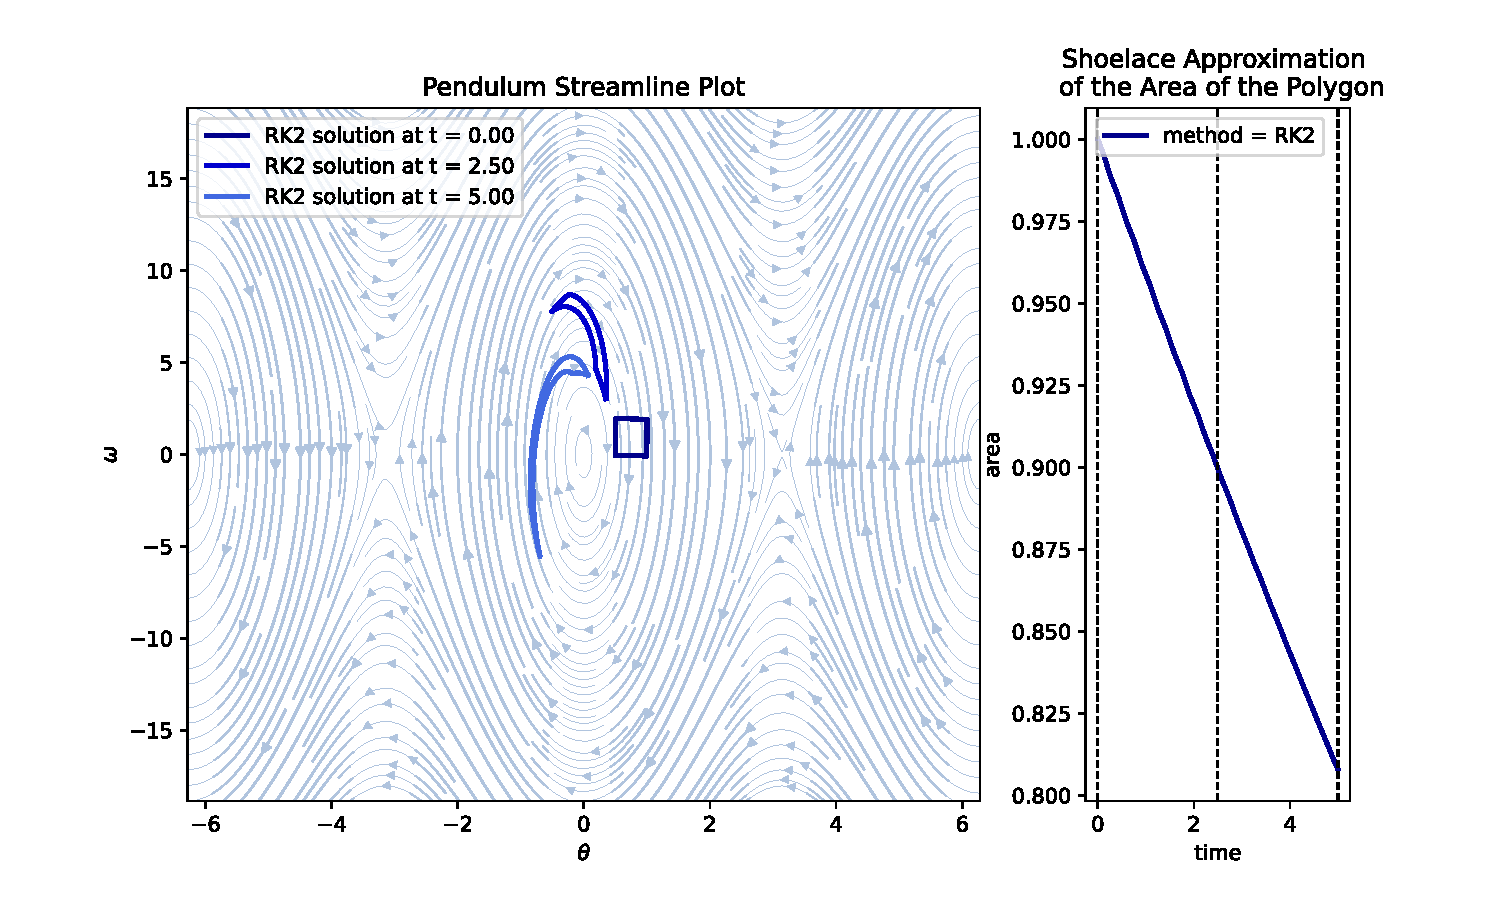
\includegraphics[width=1\textwidth]{figures/phase_spaceB.pdf}\hfill
  \caption{The left panel shows solutions to the pendulum problem at different points in time for different initial values as obtained by the RK2 scheme. The initial values are chosen so that they initially span a square in phase space. The right panel shows the phase space area spanned by the solutions as a function of time.}
  \label{fig:pend_phase_rk2}
\end{figure}

% Let us stress that a more sophisticated (non-symplectic) Runge-Kutta method would decrease the errors discussed but not change the fundamental problem of drifts in quantities that should be preserved. 
We need to switch to a whole other class of integrators.

\subsubsection{Symplectic integrators to the help}
\label{sec:symplectic_integrators}

This leads us to geometric integrators which are numerical methods preserving geometric properties of the exact flow of ODEs \citep{Hairer06}. More specifically for Hamiltonian systems we use \textbf{Symplectic Integrators} which produce a flow in phase space that is symplectic just as the flow of the exact solution \citep[chapter VI]{Hairer06}.

Symplectic integrators

\begin{itemize}
  \item are \textit{structure preserving}
  \item nearly conserve properties of Hamiltonian systems, e.g. \textit{first integrals} (variables $F(p,q)$ constant along the motion as dictated by the Hamiltonian)
  \item conserve phase-space (as prescribed by the Liouville theorem)
  \item more generally conserve all the Poincare invariants
\end{itemize}


It turns out that preserving symplecticity and energy at the same time is very difficult \citep{Hairer06b}. However, symplectic integrators still have good energy conservation properties without much long-term drifts. The general idea behind the connection between symplecticity and energy conservation is that geometric properties of the integrator (e.g. phase space conservation) translate into structure preservation on the level of modified equations \citep[preface and chapters X through XII]{Hairer06}.

\problem{Symplectic integrators do not come without caveats:
\begin{itemize}
  \item Using adaptive time-steps and keeping symplecticity is a problem.
  \item Non-conservative forces (those which cannot be described by a potential) like radiation forces (depending on velocity not only position) might be important, e.g. for debris in space and particles in planetary rings but then the central requirement of a Hamiltonian system breaks down
  \item The propagation of floating-point errors might be non-optimal
\end{itemize}
So the rebound N-body simulation package actually uses IAS15 (implicit integrator with adaptive time-stepping, 15th order) as the default \citep{Rein14}.
}

\subsubsection{Verlet Scheme}
Consider we want to solve the Newtonian equation of movement
\begin{equation}
  \partial_t^2 \vec{s} = \vec{a}(\vec{s})
\end{equation}
- a classical physical problem with a particle at position $\vec{s}$ with velocity $\vec{v}$ and an acceleration $\vec{a}$ that depends only on the position.

\note{In the following we will introduce the Störmer-Verlet, velocity Verlet and Leapfrog scheme which differ in their formulations
but are essentially the same. In molecular dynamics it is mostly called Verlet method, in the context
of partial differential equations of wave propagation leapfrog method \citep{hairer03}.}

We can derive a two-step scheme based on a Taylor expansion forward by $\Delta t$ and backward by $-\Delta t$

\begin{equation}
  \label{eq:stormer}
  \begin{aligned}
    \vec{s}(t+\Delta t) &= \vec{s}(t) + \vec{v}(t)\Delta t + \frac{1}{2} \vec{a} \Delta t^2 + \frac{1}{6} \vec{b}(t) \Delta t^3 + \mathcal{O}(\Delta t^4) \\
    \vec{s}(t-\Delta t) &= \vec{s}(t) - \vec{v}(t)\Delta t + \frac{1}{2} \vec{a} \Delta t^2 - \frac{1}{6} \vec{b}(t) \Delta t^3 + \mathcal{O}(\Delta t^4)
  \end{aligned}
\end{equation}

with

\begin{equation}
  \begin{gathered}
    \text{position } \vec{s}, \quad \text{velocity } \vec{v}, \quad \text{acceleration} \vec{a} = - \frac{1}{m} \nabla V(\vec{s}) \\
    \text{some potential } V, \quad \text{jerk } \vec{b} = \frac{d\vec{a}}{dt}
  \end{gathered}
\end{equation}

Adding both equations yields a scheme 3rd order accurate in time

\begin{equation}
  \vec{s}(t+\Delta t) = 2 \vec{s}(t) - \vec{s}(t-\Delta t) + \vec{a}(t) \Delta t^2 + \mathcal{O}(\Delta t^4)
\end{equation}

where terms with odd powers of $\Delta t$ were eliminated. This is a two-step scheme as for $\vec{s}(t+\Delta t)$, $\vec{s}(t)$ and $\vec{s}(t-\Delta t)$
are used (sometimes this form is called Störmer-Verlet).

\problem{What if we are also interested in calculating the velocity $\vec{v}$? What if $\vec{a}$ also depends on $\vec{v}$ as in the Lorentz and we need $\vec{v}$ to calculate $\vec{a}$?}

From subtracting the equations \ref{eq:stormer}, we can find
\begin{equation}
  \vec{v}(t) = \frac{\vec{s}(t+\Delta t) - \vec{s}(t - \Delta t)}{2 \Delta t} - \frac{1}{6} \vec{b}(t) \Delta t^2 + \mathcal{O}(\Delta t^3)
\end{equation}
but this is problematic as
\begin{itemize}
  \item \textcolor{red1}{only accurate to the third order}
  \item \textcolor{red1}{an implicit equation as we do not know the future $\vec{s}(t+\Delta t)$ at the current timepoint}
  \item \textcolor{red1}{we would need to know the jerk at the current timestep which could itself depend on $\vec{v}(t)$}, \textcolor{green1}{we could
  ignore the jerk}, \textcolor{red1}{but then the accuracy is only $\mathcal{O}(\Delta t^2)$}
\end{itemize}

\subsubsubsection{Velocity Verlet algorithm}
\idea{Starting again from the Taylor expansion, we omit the jerk and extrapolate the velocity $\vec{v}(t+\Delta t)$ using the average of the
accelerations at $t$ and $t + \Delta t$}
\begin{equation}
  \begin{aligned}
    \vec{s}(t+\Delta t) &= \vec{s}(t) + \vec{v}(t) \Delta t + \frac{1}{2} \vec{a} \Delta t^2 +  \mathcal{O}(\Delta t^3) \\
    \vec{v}(t+\Delta t) &= \vec{v}(t) + \frac{\vec{a}(t) + \vec{a}(t + \Delta t)}{2} + \mathcal{O}(\Delta t^2)
  \end{aligned}
\end{equation}
\note{Again, we use $\vec{a}(t + \Delta t)$ to get $\vec{v}(t+\Delta t)$ which is not possible if $\vec{a}$ depends on $v$. If we would take only $\vec{a}(t)$
instead of the average, we would just have explicit Euler.}
In steps we can write
\begin{enumerate}
  \item calculate the new position: $\vec{s}(t+\Delta t) = \vec{s}(t) + \vec{v}(t)\Delta t + \frac{1}{2} \vec{a}(t) \Delta t^2$
  \item update the acceleration: $\vec{a}(t+\Delta t) = -\frac{1}{m} \left. \nabla V \right|_{\vec{s}(t+\Delta t)}$
  \item calculate the new velocity: $\vec{v}(t+\Delta t) = \vec{v}(t) + \frac{\vec{a}(t) + \vec{a}(t+\Delta t)}{2} \Delta t$
  \item update the time: $t \rightarrow t + \Delta t$
\end{enumerate}
Introducing half timesteps, we can write the Verlet scheme as a combination of 1st order steps
\begin{enumerate}
  \item $\vec{v}\left( t + \frac{1}{2} \Delta t \right) = \vec{v}(t) + \frac{1}{2} \vec{a}(t) \Delta t$
  \item $\vec{s}(t + \Delta t) = \vec{s}(t) + \vec{v}\left( t + \frac{1}{2}\Delta t \right) \Delta t$\\(note that plugging (1) into (2) yields the previous step (1))
  \item $\vec{a}(t+\Delta t) = -\frac{1}{m} \left. \nabla V \right|_{\vec{s}(t+\Delta t)}$
  \item $\vec{v}\left( t + \Delta t \right) = \vec{v}\left( t + \frac{1}{2} \Delta t \right) + \frac{1}{2} \vec{a}(t+\Delta t) \Delta t$\\(note that plugging (1) into (4) yields the previous step (3))
  \item $t \rightarrow t + \Delta t$
\end{enumerate}
This is illustrated in figure \ref{fig:vel_verl}. Here the last step can be called \textit{implicit} as it depends on $\vec{a}(t+\Delta t)$, so a result at the same time as it is supposed
to deliver a result at - we have a semi-implicit Euler scheme.

\begin{figure}[!htb]
  \centering
  \includesvg[width=0.9\textwidth]{figures/vel_verl_2.svg}\hfill
  \caption{Illustration of the velocity Verlet scheme.}
  \label{fig:vel_verl}
\end{figure}

\subsubsection{The Leapfrog Method}
We will now introduce the Leapfrog scheme and at its hand what it means for a method to be symplectic.

The leapfrog scheme can then be written as
\begin{equation}
\begin{aligned}
& \vec{s}(t + \frac{1}{2} \Delta t)=\vec{s}(t - \frac{1}{2} \Delta t)+ \vec{v}(t) \Delta t + \mathcal{O}(\Delta t^3) \\
& \vec{v}(t + \Delta t)=\vec{v}(t)+ \vec{a}(t + \frac{1}{2} \Delta t) \Delta t  + \mathcal{O}(\Delta t^2)
\end{aligned}
\end{equation}

The position and velocity are updated at alternating half time steps as illustrated in figure \ref{fig:leapfrog},
just as the name suggests (the velocity is "leaping" over the position and vice versa (\textit{Bockspringen})).

\begin{figure}[!htb]
  \centering
  \includesvg[width=0.9\textwidth]{figures/lf.svg}\hfill
  \caption{Illustration of the leapfrog scheme.}
  \label{fig:leapfrog}
\end{figure}

\note{To start the scheme or to save the position and velocity at the same time, a half step needs to be performed, e.g. using half standard explicit Euler.}

\subsubsubsection{Connection between Leapfrog and Velocity Verlet}
We can combine steps $4,5,1$ in the velocity Verlet scheme in the half-step formulation to get
\begin{equation}
  \begin{aligned}
    & \vec{s}(t + \Delta t) = \vec{s}(t) + \vec{v}\left( t + \frac{1}{2} \Delta t \right) \Delta t \\
    & \vec{v}(t + \frac{3}{2} \Delta t) =\vec{v}(t + \frac{1}{2} \Delta t) + \vec{a}(t + \Delta t) \Delta t
    \end{aligned}
\end{equation}
which if we shift everything by $\frac{1}{2} \Delta t$ yields the aforementioned leapfrog scheme. Phrased differently
velocity Verlet is leapfrog with Euler-kickoff built-in.

\subsubsubsection{Kick-drift-kick and Drift-kick-drift Leapfrog formulations to have velocity and position information at the same time}
\problem{One problem of the Leapfrog scheme in this form is that velocity and position information are not available at the same time. This is for instance problematic
if we want to calculate the energy which depends on both or if we want to change the step-size adaptively without destryoing the interlacement (see figure \ref{fig:leapfrog_adaptive_problem}).}
\idea{We rearrange and split the interlaced integration by a full time step into a half step in first variable, full step in second variable, half step in first variable.}

There are two possible schemes.

\begin{figure}[!htb]
  \centering
  \includesvg[width=0.9\textwidth]{figures/leapfrog_adaptive.svg}\hfill
  \caption{Illustration of the problem of changing the step-size in the leapfrog scheme and the solutions - kick-drift-kick and drift-kick-drift.}
  \label{fig:leapfrog_adaptive_problem}
\end{figure}

In the \textbf{kick-drift-kick formulation}, positions are stored at full, velocities at half time steps (equivalent to the velocity Verlet).

\begin{equation}
\begin{aligned}
& \vec{v}(t + \frac{1}{2} \Delta t)=\vec{v}(t)+ \vec{a}(t) \frac{\Delta t}{2}  \quad \text {kick, half-step in first variable}\\
& \vec{s}(t + \Delta t)=\vec{s}(t)+ \vec{v}(t + \frac{1}{2} \Delta t) \Delta t  \quad \text {drift, full-step in second variable}\\
& \vec{v}(t + \Delta t)=\vec{v}(t + \frac{1}{2} \Delta t)+ \vec{a}(t + \Delta t) \frac{\Delta t}{2}  \quad \text {kick, half-step in first variable}\\
& \text{possibly adapt step-size here}\\
& t \rightarrow t + \Delta t
\end{aligned}
\end{equation}

where a \textit{drift} is a change of the position with constant velocity and a \textit{kick} is a change of the velocity with constant acceleration.

In the \textbf{drift-kick-drift formulation}, velocities are stored at full, positions at half time steps.

\begin{equation}
\begin{aligned}
& \vec{s}(t + \frac{1}{2} \Delta t)=\vec{s}(t)+ \vec{v}(t) \frac{\Delta t}{2}  \quad \text {drift, half-step in first variable}\\
& \vec{v}(t + \Delta t)=\vec{v}(t)+ \vec{a}(t + \frac{1}{2} \Delta t) \Delta t  \quad \text {kick, full-step in first variable}\\
& \vec{s}(t + \Delta t)=\vec{s}(t + \frac{1}{2} \Delta t)+ \vec{v}(t + \Delta t) \frac{\Delta t}{2} \quad \text {drift, half-step in first variable}\\
& \text{possibly adapt step-size here}\\
& t \rightarrow t + \Delta t
\end{aligned}
\end{equation}

\subsubsubsection{Advantages of the Leapfrog scheme}

The leapfrog scheme is second order accurate, symmetric (time reversible), symplectic, has good energy conservation properties and is time reversible (proofs in \cite[chapter 2.8]{springel23}).

Second order accuracy may be surprising as we seemingly only Taylor approximate up to the first order - but note the interlacement
and connection to velocity Verlet.

\subsubsubsection{Leapfrog is time-symmetric and reversible}
In terms of the one-step map $\Phi_h: (\vec{s}_n, \vec{v}_n) \rightarrow (\vec{s}_{n+1}, \vec{v}_{n+1})$ time-symmetry means that $\Phi_{-\Delta t}^{-1} = \Phi_{\Delta t}$
so going one step and one back by switching the direction of time leads us back to where we came from, $n \rightleftharpoons n + 1$.

We integrate from $\left( \vec{s}_n, \vec{v}_{n-\frac{1}{2}} \right)$ to $\left( \vec{s}_{n+1}, \vec{v}_{n+\frac{1}{2}} \right)$ and see that changing $\Delta t \rightarrow -\Delta t$ and going a step leads us back to the initial state.

\begin{equation}
  \begin{gathered}
  \vec{s}_{\text{fin}}=\mathcolor{green1}{\vec{s}_{n+1}}-\vec{v}_{n+\frac{1}{2}} \Delta t=\mathcolor{green1}{\vec{s}_n+\vec{v}_{n+\frac{1}{2}} \Delta t}-\vec{v}_{n+\frac{1}{2}} \Delta t=\vec{s}_n \\
  \vec{v}_{\text{fin}}=\mathcolor{green1}{\vec{v}_{n+\frac{1}{2}}}-\vec{a}_n \Delta t=\mathcolor{green1}{\vec{v}_{n+\frac{1}{2}}+\vec{a}_n \Delta t}-\vec{a}_n \Delta t=\vec{v}_{n-\frac{1}{2}}
  \end{gathered}
\end{equation}

\greenbox{The flow is also reversible - inverting the direction of initial velocity does not change
the solution trajectory, it just inverts the direction (if the acceleration only depends on the position).}

\pinkbox{\textbf{Reversibility}:
A system of differential equations
\begin{equation*}
  \begin{aligned}
    \partial_t \vec{s} &= \vec{f}(\vec{s},\vec{v}) \\
    \partial_t \vec{v} &= \vec{g}(\vec{s},\vec{v})
  \end{aligned}
\end{equation*}
is reversible if
\begin{equation*}
  \begin{aligned}
    \vec{f}(\vec{s},-\vec{v}) &= -\vec{f}(\vec{s},\vec{v}) \\
    \vec{g}(\vec{s},-\vec{v}) &= \vec{g}(\vec{s},\vec{v})
  \end{aligned}
\end{equation*}
such that the time development map $\phi_t$ fulfills
\begin{equation*}
  \phi_t(\vec{s},\vec{v}) = (\vec{\hat{s}},\vec{\hat{v}}) \quad \text{implies} \quad \phi_{t}(\vec{\hat{s}},-\vec{\hat{v}}) = (\vec{s},-\vec{v})
\end{equation*}
- so reflecting the velocity at any point on the trajectory, lets us move back along the trajectory. \textbf{The leapfrog
scheme is reversible} as of
\begin{equation*}
  \Phi_{\Delta t}(\vec{s}, \vec{v}) = (\vec{\hat{s}}, \vec{\hat{v}}) \quad \text{implies} \quad \Phi_{-\Delta t}(\vec{s}, -\vec{v}) = (\vec{\hat{s}}, -\vec{\hat{v}})
\end{equation*}
(which holds for most numerical schemes) and time-symmetry $\Phi_{-\Delta t}^{-1} = \Phi_{\Delta t}$.
}

So leapfrog is time-symmetric and reversible, different from e.g. explicit Euler (see figure \ref{fig:euler_symm}).

\begin{figure}[!htb]
  \centering
  \includesvg[width=0.5\textwidth]{figures/euler_symm.svg}\hfill
  \caption{Explicit Euler is not symmetric (time-reversible).}
  \label{fig:euler_symm}
\end{figure}

\greenbox{\textbf{Advantages of symmetric methods}: Symmetric methods
applied to \textit{integrable and near-integrable} \textbf{reversible systems} share
similar properties to symplectic methods applied to \textit{(near)-integrable} Hamiltonian
systems: linear error growth and long-time near-conservation of first integrals.
\textcolor{red1}{For a non-reversible system, a symmetric but non-symplectic method (e.g. Lobatto IIIB) will have 
no good conservation properties though.}}

\note{Not every symplectic method is symmetric. For instance symplectic Euler is symplectic but not symmetric.}

\subsubsubsection{Symplecticity of the leapfrog scheme I: Intuition and Meaning}
Symplecticity (so area conservation in phase space) is illustrated at the hand of the pendulum in figure \ref{fig:pend_phase_lf} and energy conservation at the hand of the two-body-problem in figure \ref{fig:leapfrog_orbit}. The area in phase space does not change at all while the energy shows small fluctuations but no overall drift (compare \cite[theorem 5.5]{hairer03}). The angular momentum is exactly conserved in the leapfrog solution to the two-body-problem (details on the conservation of specific \textit{quadratic first integrals} can be found in \cite[theorem 3.5]{hairer03}). As visible in the changing orientation of the orbit in figure \ref{fig:leapfrog_orbit} the leapfrog scheme does not preserve the orientation of the Runge-Lenz vector.

\begin{figure}[!htb]
  \centering
  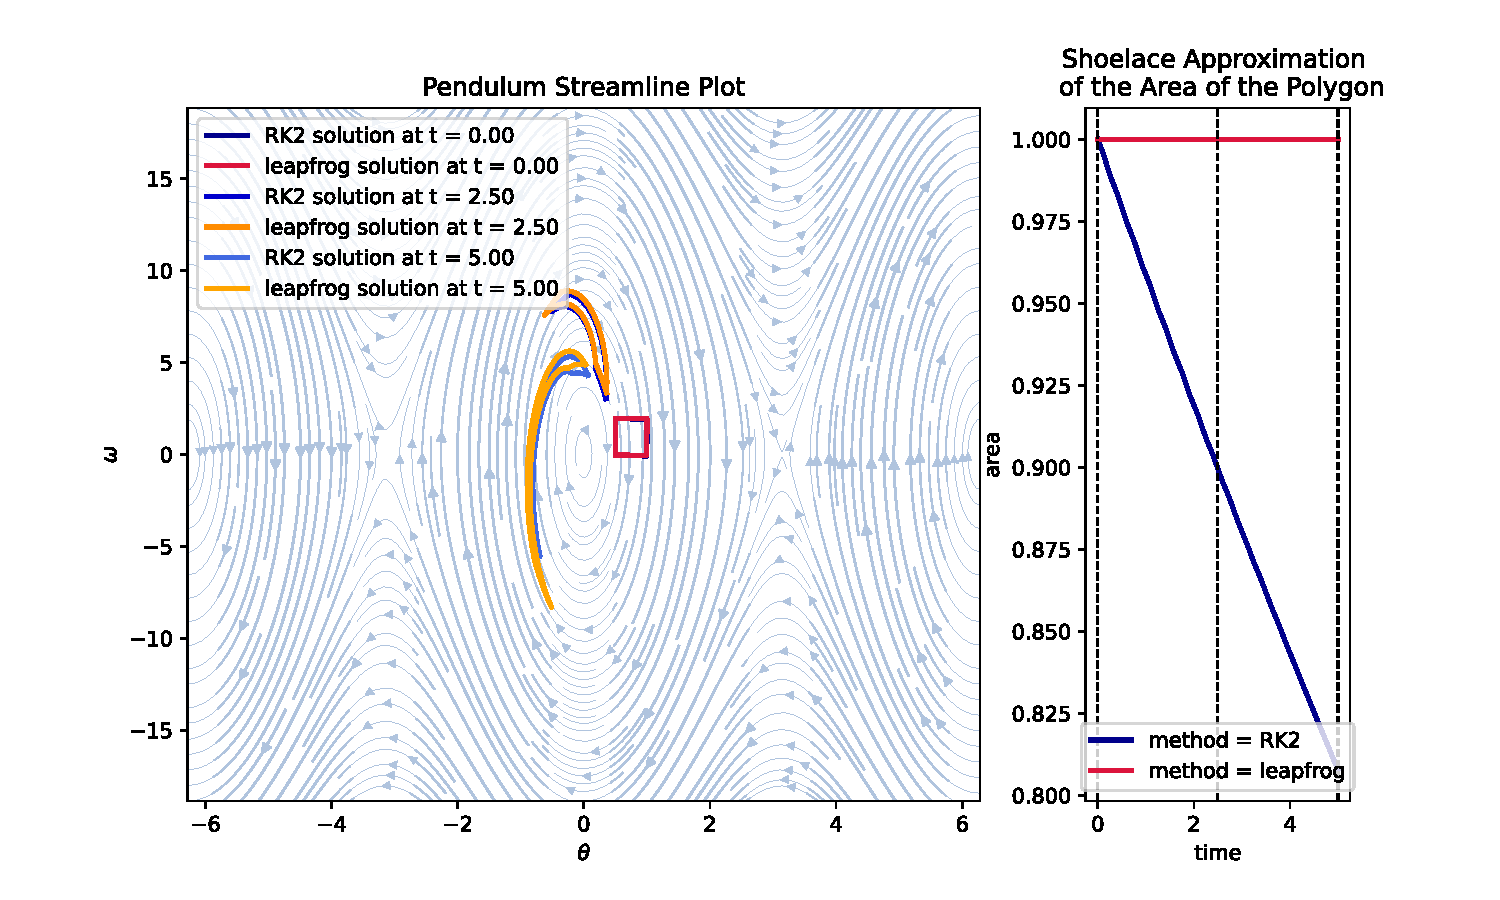
\includegraphics[width=1\textwidth]{figures/phase_spaceA.pdf}\hfill
  \caption{The same situation as in figure \ref{fig:pend_phase_rk2} is shown but now with the result of the leapfrog method added. The leapfrog scheme preserves the area in phase space while the RK2 scheme does not.}
  \label{fig:pend_phase_lf}
\end{figure}

\begin{figure}[!htb]
  \centering
  \includesvg[width=1\textwidth]{figures/grav_orbit_Leapfrog.svg}\hfill
  \caption{Numerical solution of the two-body-problem using the leapfrog method in the kick-drift-kick scheme. The left panel shows the orbit, the central one the energy and the right one the angular momentum. Time is also encoded in the form of color, going from a dark blue to yellow.}
  \label{fig:leapfrog_orbit}
\end{figure}

\subsubsubsection{Symplecticity of the leapfrog scheme II: Proof}
Consider the separable Hamiltonian
\begin{equation}
  \begin{aligned}
    H(q,p) &= H_{\text{kin}}(p) + H_{\text{kin}}(q) \\
           &\explain{=}{here} \frac{p^2}{2m} + U(q)
  \end{aligned}
\end{equation}
\textcolor{blue1}{Procedure}: We solve both parts of the Hamiltonian separately (operator splitting) and construct Leapfrog as
the concatenation of these solutions (proving symplecticity) and then calculate an error Hamiltonian.

\paragraph{Operator splitting} From the Hamiltonian equations of the kinetic and potential part, we find update steps.

For the kinetic part $H_{\text{kin}}$ we find

\begin{equation}
  \left.\begin{array}{c}
  \partial_t q=\partial_p H_{\text{kin}}=\frac{p}{m} \\
  \partial_t p=-\partial_q H_{\text{kin}}= 0
  \end{array}\right\} \rightarrow\left\{\begin{array}{c}
  q^{(n+1)}=q^{(n)}+\frac{p^{(n)}}{m} \Delta t \\
  p^{(n+1)}=p^{(n)}
  \end{array}\right.
\end{equation}

and for the potential part

\begin{equation}
  \left.\begin{array}{c}
  \partial_t q=\partial_p H_{\text{pot}}=0 \\
  \partial_t p=-\partial_q H_{\text{pot}}= -\partial_q U
  \end{array}\right\} \rightarrow\left\{\begin{array}{c}
  q^{(n+1)}=q^{(n)} \\
  p^{(n+1)}=p^{(n)} - \partial_q U \Delta t
  \end{array}\right.
\end{equation}

\note{Independent of $\Delta t$ the schemes found are exact; and symplectic as brought forward by Hamiltonians.}

\paragraph{Constructing leapfrog} Let $\phi_{\Delta t}(H)$ describe making a step $\Delta t$ governed by $H$ in phase-space
(a time evolution operator). Then leapfrog (kick-drift-kick version) is given as
\begin{equation}
  \phi_{\Delta t}(H) = \phi_{\frac{\Delta t}{2}}(H_{\text{pot}}) \odot \phi_{\Delta t}(H_{\text{kin}}) \odot \phi_{\frac{\Delta t}{2}}(H_{\text{pot}})
\end{equation}
\textcolor{blue1}{so Leapfrog is symplectic as a concatenation of symplectic operators}, so
\begin{itemize}
  \item there is no secular (long-lasting, non-oscillatory) drift in e.g. the Energy of e.g. the Kepler orbits
  \item the longer the timespan to simulate, the more it makes sense to use leapfrog over Runge Kutta schemes (e.g. the explicit Euler scheme always overshoots the orbits leading to increasing total energy and unbound states)
\end{itemize}

\note{\enquote{Yes, symplectic integrators do not exactly conserve energy. It is a common misconception that they do. What symplectic integrators actually do is solve for a trajectory which rests on a symplectic manifold that is perturbed from the true solution's manifold by the truncation error. This means that symplectic integrators do not experience (very much) longtime drift, but their orbit is not exactly the same as the true solution in phase space, and thus you will see differences in energy that tend to look periodic. There is a small drift which grows linearly and is related to floating-point error, but this drift is much less than standard methods. This is why symplectic methods are recommended for longtime integration.} \citep{rackauckas22}}

\paragraph{Error Hamiltonian} Indeed, it turns out that the leapfrog scheme exactly solves the modified Hamiltonian

\begin{equation}
  H_{leap} = H + H_{err}, \quad H_{err} \propto \frac{\Delta t^2}{12} \left\{ \left\{ H_{kin}, H_{pot} \right\}, H_{kin} + \frac{1}{2} H_{pot}\right\} + \mathcal{O}(\Delta t^3)
\end{equation}

where $H_{kin}$ and $H_{pot}$ are the kinetic and potential part of the original Hamiltonian \citep[chapter 2.8]{springel23}. The curly brackets denote the Poisson bracket.

\paragraph{Notes on the derivation of the Error Hamiltonian} The time evolution of a phase space
function $F(p,q)$ under the flow generated by a Hamiltonian $H$ fulfills $-\partial_t F = -\{ H, F \} = - \hat{H} F$
and similar to the time-development operator in Quantum Mechanics, we can write

\begin{equation}
  F(t) = \exp{\left( \hat{H}t \right)} F(0)
\end{equation}

and for the leapfrog scheme with $H_{leap} = H + H_{err}, H = H_{kin} + H_{pot}$ we have

\begin{equation}
  \exp \left(\left(H+H_{\text {err }}\right) \Delta t\right)=\exp \left(H_{\text {pot }} \frac{\Delta t}{2}\right) \exp \left(H_{\text {kin }} \Delta t\right) \exp \left(H_{\text {pot }} \frac{\Delta t}{2}\right)
\end{equation}

where using the the Baker-Campbell-Hausdorff formula lets us find $H_{\text {err}}$.

\subsection{Extrapolation method: Bulirsch-Stoer algorithm}
Our goal is still to obtain highly accurate and cheap solutions
to ODEs. The ingedriends of Bulirsch-Stoer are
\begin{enumerate}
  \item we integrate across a whole interval with length $H$ multiple times with a sequence of decreasing substep-sizes $h_j$ each yielding a final result $F(h_j)$
  \item we extrapolate $F(h)$ to $h = 0$ asking ourselves \textit{What would be the solution, if we had taken infinitely many, infinitely small steps?}, for instance using polynomial extrapolation or Richardson extrapolation\footnote{A sequence acceleration method to based on a sequence $F(h)$ for decreasing $h$ extrapolate to $h = 0$.}
\end{enumerate}
with the method being most-appropriate for differential equations containing smooth (cheap to evaluate) functions. An illustration is given in figure \ref{fig:bulirsch_stoer}.

\begin{figure}[!htb]
  \centering
  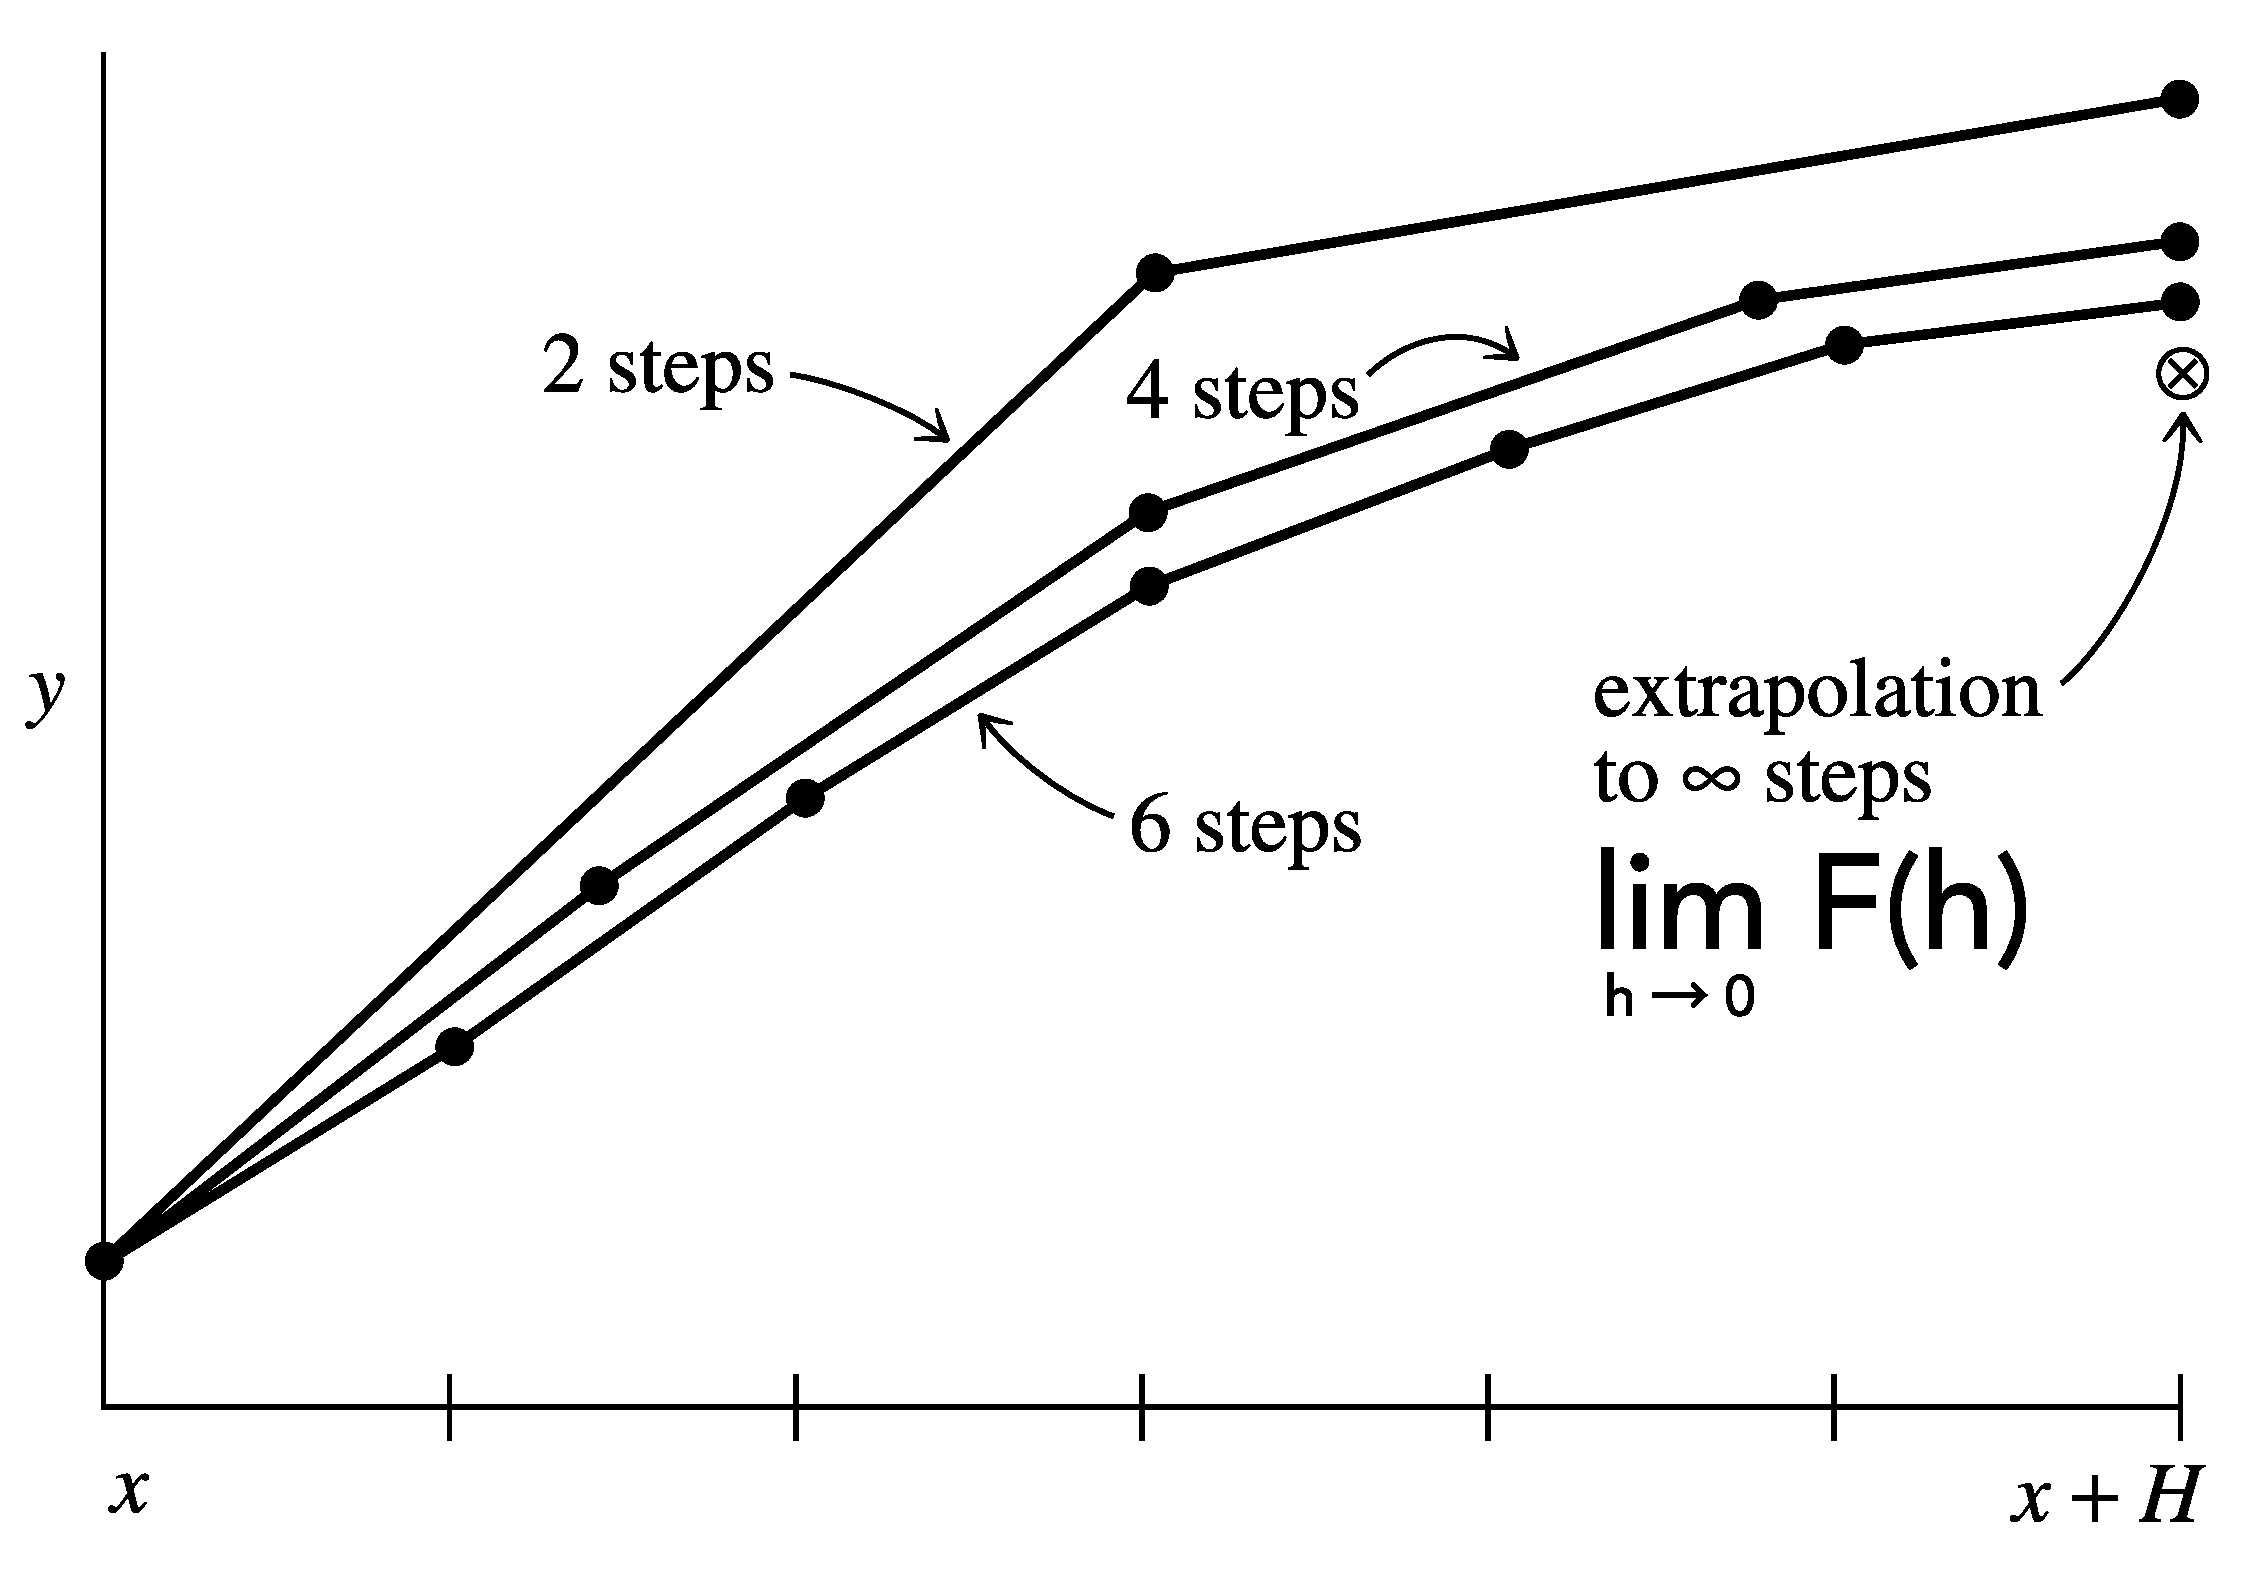
\includegraphics[width=0.9\textwidth]{figures/bulirsch.pdf}\hfill
  \caption{Illustration of the Bulirsch-Stoer algorithm.}
  \label{fig:bulirsch_stoer}
\end{figure}

\redbox{While the idea of this method is very beautiful, its usage is disputed, with e.g. W. Van Snyder \href{https://www.stat.uchicago.edu/~lekheng/courses/302/wnnr/nr.html}{writing}: extrapolation methods are almost always substantially inferior to Runge-Kutta, Taylor's series, or multistep methods.}

A single step taking us from $x$ to $x+H$ (large distance $H$) consists of many substeps using the modified midpoint rule.

\subsubsection{Basic integration method | second order method with $\mathcal{O}(h^2)$; midpoint rule $\rightarrow$ modified midpoint rule}
The midpoint rule is given by
\begin{equation}
  \begin{aligned}
    k_1 &= f(y_i,x_i) \\
    k_2 &= f\left( y_i + \frac{h}{2} k_1, x_i + \frac{h}{2} \right) \\
    x_{i+1} &= x_i + h \\
    y_{i+1} &= y_i + h k_2 + \mathcal{O}(h^3)
  \end{aligned}
\end{equation}
as illustrated in figure \ref{fig:midpoint_rule}.

\begin{figure}[!htb]
  \centering
  \includesvg[width=0.9\textwidth]{figures/midpoint.svg}\hfill
  \caption{Illustration of the midpoint rule.}
  \label{fig:midpoint_rule}
\end{figure}

\subsubsubsection{Modified midpoint rule}
We advance from $x$ to $x + H$ using $n$ substeps of size $h = \frac{H}{n}$. Except for the first and
last step, we advance using the midpoint rule.
\greenbox{\textbf{Advantage of the midpoint rule over RK2:} We only need one evaluation of $f$ per step $h$ instead of two.}

\begin{equation}
  \vcenter{\hbox{\begin{minipage}{0.2\textwidth}
  \centering
  \includesvg[width=\textwidth]{figures/modified_midpoint.svg}
  \captionof{figure}{Modified midpoint rule.}
  \end{minipage}}}
  \qquad\qquad
  \begin{aligned}
      z_0 &= y(x) \\
      z_1 &= z_0 + h f(z_0, x) \text{ not midpoint}\\
      z_2 &= z_0 + 2h f(z_1, x + h) \text{ midpoint with stepsize } 2h\\
      z_3 &= z_1 + 2h f(z_2, x + 2h) \text{ midpoint with stepsize } 2h\\
      \vdots \\
      z_m &= z_{m-2} + 2hf(z_{m-1},x+(m-1)h) \\
      z_{m + 1} &= z_{m-1} + 2hf(z_{m},x+mh), \quad m=4,\dots,n-1 \\
      \vdots \\
      y(x+H) &\approx y_n = \frac{1}{2} \left[ z_n + \explain{z_{n-1} + hf(z_n,x+H)}{euler Step from $z_{n-1}$} \right]
  \end{aligned}
\end{equation}
\subsubsubsection{Combining modified midpoint calculations with different $h$; advantage of modified midpoint}
Remember that the midpoint rule is of 2nd order so the error when covering an interval $H$ with multiple steps
is $\mathcal{O}(h^2)$. Central to the advantage of the modified midpoint rule is (not proven here)
\begin{equation}
  y(x+H) - y_n = \sum_{i=1}^{\infty} \alpha_i h^{2i}
\end{equation}
so the error between the true $y(x+H)$ and our numerical result $y_n$ expressed as a power
series in $h$ only contains even powers of $h$. \textcolor{green1}{We can therefore combine results
with different step-sizes to gain two oders at a time}.
\paragraph{Example} Let us combine a version with $n$ steps $h$ and one with $2n$ steps $2h$.
\begin{equation}
  \begin{aligned}
    n:& \quad y(x+H) - y_n = \alpha_1 h^2 + \alpha_2 h^4 \\
    2n:& \quad y(x+H) - y_{2n} = \alpha_1 \left( \frac{h}{2} \right)^2 + \alpha_2 \left( \frac{h}{2} \right)^4
  \end{aligned}
\end{equation}
from which we obtain
\begin{equation}
  y(x + H) = \frac{4y_{2n}-y_n}{3} + \mathcal{O}(h^4)
\end{equation}
which is 4th order accurate like RK4 but at less cost (function evaluations).
\subsubsubsection{What extrapolation nodes to choose? - how to inrease $n$ (or rather decrease $h$)}
Let us remember
\begin{equation}
  F(h_n) = y_n \quad \text{with } n = \frac{H}{h}
\end{equation}
We cross the large interval $H$ using multiple substeps multiple times with decreasing substep size. Each iteration
delivers a result $F(h_n)$ and we have already seen that such results can be combined smartly - and extrapolation
to $h\rightarrow 0$ is even better. But what evalutation nodes for $F(h)$ should we choose?
\begin{equation}
  \begin{aligned}
    \text{Romberg}:& \quad n = [2,4,8,16,\dots,1024] \\
    \text{Bulirsch}:& \quad n = [2,4,6,8,12,16,\dots,96] \\
    \text{Deufelhard}:& \quad n = [2,4,6,8,10,\dots,24]
  \end{aligned}
\end{equation}
\subsubsubsection{How to extrapolate from multiple $F(h_n)$ to the limit $h\rightarrow 0$?}
One option is polynomial interpolation (two points define a line, ..., $n$ points define
a polynomial of (max) degree $n-1$), so we do polynomial regression and evaluate it at zero.

There is also the approach to use rational functions,
which can also capture poles and divergence regions between the interpolation points (which 
polynomials will never do), so
\begin{equation}
  R_{m+1}(x)=\frac{P_\mu(x)}{Q_\nu(x)}=\frac{p_0+p_1 x+p_2 x^2+\cdots+p_\mu x^\mu}{q_0+q_1 x+q_2 x^2+\cdots+q_v x^v}, \quad m+1=v+\mu+1
\end{equation}

\redbox{\cite{hairer93} write: \enquote{Many authors in the sixties claimed that it is better to use rational functions instead of polynomials. Later numerical experiments (Deuflhard 1983) showed that rational extrapolation is nearly never more advantageous than polynomial extrapolation.}. 
One reason I can imagine is that the more complex rational model is more unstable and harder to appropriately fit.}

\pinkbox{\textbf{Richardson extrapolation:} Consider generally
\begin{equation}
  F(h) = F^\star + \alpha h^{k_0} + \mathcal{O}(h^{k_1}), \quad k_0 < k_1
\end{equation}
and based on a sequence $F(h)$ for decreasing $h$ we want to extrapolate to $h = 0$, so to $F^\star$. As an
example consider $k_0 = p$, $k_1 = p + 1$. Then $R(h,\beta)$ with
\begin{equation}
  R(h,\beta) = \frac{\beta^p F(h \slash \beta) - F(h)}{\beta^p - 1} = F^\star + \mathcal{O}(h^{p+1})
\end{equation}
is called a Richardson extrapolation, which is a higher order estimate.
}

\subsection{Predictor-corrector methods}
\greenbox{\textbf{Multistep idea}: While a one-step method only uses the differential value and the ODE itself in a step, multistep methods also
include information from previous steps (e.g $x,x-h,x-2h$) to obtain better estimates for the next step
($x+h$). The method is e.g. kicked off using Runge-Kutta steps.}

Let us start by writing an advance in an ODE $\partial_x y = f(y(x),x)$ as
\begin{equation}
  y_{n+1} = y_n + \int_{x_n}^{x_{n+1}} f(x',y(x')) dx'
\end{equation}
the problem is that different from an integration problem, we would need
to know $y(x)$ to use this formula to calculate $y(x)$ or rather $y_{n+1}$ - so what have we won?

Consider we are in the multistep setting and already have approximations $y_n,y_{n-1},\dots$
at $x_n,x_{n-1},\dots$. We can then approximate $f(x,y)$ by a polynomial passing through those
points and yield
\begin{equation}
  \label{eq:fix}
  y_{n+1} = y_n + h\cdot (\beta_0 f(x_{n+1},y_{n+1}) + \beta_1 f(x_{n},y_{n}) + \beta_2 f(x_{n-1},y_{n-1}) + \dots)
\end{equation}
But wait - we used $y_{n+1}$ in the RHS which we do not know. We could get an explicit scheme by setting $\beta_0 = 0$
but the formula screams fixpoint iteration (as in Picard iteration) - \textbf{predictor-corrector method}.
\begin{enumerate}
  \item \textbf{predictor step:} obtain a good estimate for $y_{n+1}$
  \item \textbf{corrector step(s):} plugging the result of the predictor step into eq. \ref{eq:fix} gives an improved estimate for $y_{n+1}$
\end{enumerate}
For correction to make sense, the first prediction must be sufficiently good.

\subsubsection{One-step predictor-corrector method: RK2 and $P(EC)^k$}
Indeed standard RK2 is a predictor-corrector method
\begin{equation}
  \begin{gathered}
    k_1=f\left(y_{n}, x_{n}\right) \\
    k_2=f\left(\explain{y_{n}+h k_1}{predictor}, x_n+h\right) \\
    \explain{y_{n + 1}=y_{n}+\frac{h}{2}\left(k_1+k_2\right)+\mathcal{O}\left(h^3\right)}{corrector}
  \end{gathered}
\end{equation}
\paragraph{Different notation and $P(EC)^k$ method} We write the predictor P step as
\begin{equation}
  \tilde{y}_{n+1,[0]}^{P} = y_n + hf(y_n,x_n)
\end{equation}
and can then write the evaluation / corrector step EC as
\begin{equation}
  \tilde{y}_{n+1,[1]}^{EC} = y_n + \frac{h}{2} \left[ f(y_n,x_n) + f(\tilde{y}_{n+1,[0]}^{P},x_{n+1}) \right]
\end{equation}
which we can repeat
\begin{equation}
  \begin{aligned}
    \tilde{y}_{n+1,[2]}^{EC} &= y_n + \frac{h}{2} \left[ f(y_n,x_n) + f(\tilde{y}_{n+1,[1]}^{EC},x_{n+1}) \right] \\
    \tilde{y}_{n+1,[k]}^{EC} &= y_n + \frac{h}{2} \left[ f(y_n,x_n) + f(\tilde{y}_{n+1,[k-1]}^{EC},x_{n+1}) \right]
  \end{aligned}
\end{equation}
until convergence $|\tilde{y}_{n+1,[k]}^{EC} - \tilde{y}_{n+1,[k-1]}^{EC}| \leq \epsilon_0$ (some error tolerance $\epsilon_0$) where
our final approximation is $y_{n+1} = \tilde{y}_{n+1,[k]}^{EC}$. This is the $P(EC)^k$ method.

\subsubsection{4th order Adams-Bashforth-Moulton}
Here we used the multistep principle as introduces above. In the 4th order Adams-Bachforth-Moulton approach
we use three previous timesteps. It is a 4th order method.

The predictor step has weights designed so it gives the correct result for cubic polynomials
\begin{equation}
  \tilde{y}_{n+1} = y_n + \frac{h}{24} \left[ 55 f(y_n,x_n) - 59 f(y_{n-1},x_{n-1}) + 37 f(y_{n-2},x_{n-2}) - 9 f(y_{n-3},x_{n-3}) \right] + \mathcal{O}(h^5)
\end{equation}
the evaluation / corrector step EC is
\begin{equation}
  y_{n+1} = y_n + \frac{h}{24} \left[ 9 f(\tilde{y}_{n+1},x_{n+1}) + 19 f(y_{n},x_{n}) - 5 f(y_{n-1},x_{n-1}) + f(y_{n-2},x_{n-2}) \right] + \mathcal{O}(h^5)
\end{equation}
containing $\tilde{y}_{n+1}$ (\textit{implicit}) and can be repeated for higher accuracy (plug in $y_{n+1}$ instead of $\tilde{y}_{n+1}$ in the next EC step). We start the scheme with three RK steps.

\subsection{Shooting | adapting parameters until boundary conditions are fulfilled}
\subsubsection{Remark on ODE solutions in phase space}
There are infinitely many solutions to an ODE but only one unique to a initial value problem. Those
solutions are streamlines through phase space that
\begin{itemize}
  \item do not start / end
  \item do not cross
\end{itemize}
\subsubsection{Examplary Shooting Problem}
Consider the motion of a projectile from a canon, given by
\begin{equation}
  \partial_t^2 \begin{pmatrix} x \\ y \end{pmatrix}= \begin{pmatrix} 0 \\ -g \end{pmatrix} - b \partial_t \begin{pmatrix} x \\ y \end{pmatrix}
\end{equation}
where the canon sits at $(0,1)$ and shoots with a give velocity $v_{\text{canon}}$ at an angle $\alpha$ to the horizontal. Our
aim is hitting a target at $(x_{\text{target}},y_{\text{target}})$ (boundary condition). This is illustrated in figure \ref{fig:shooting_problem}.

\begin{figure}[!htb]
  \centering
  \includesvg[width=0.9\textwidth]{figures/shooting.svg}\hfill
  \caption{Illustration of the shooting problem. Trajectories gained by converting the system to first order ($\vec{q} = (x,y,v_x,v_y), f = (v_x,v_y,-bv_x,-g-bv_y)$) and then applying RK2.}
  \label{fig:shooting_problem}
\end{figure}
  
\subsubsection{Shooting}
In the shooting method a boundary value problem is reduced to an initial value problem. We solve the initial value problem 
for different choices of parameters 
until the given boundary conditions 
are satisfied – \textcolor{blue1}{we shoot trajectories in different directions from one boundary until we find one that hits the other boundary condition}.
For a neutron star we could know the central density and density at the surface and seek some process parameters.

\pagebreak